% !TeX spellcheck = en-US
% !TeX encoding = utf8
% !TeX program = pdflatex
% !BIB program = biber
% -*- coding:utf-8 mod:LaTeX -*-


% vv  scroll down to line 200 for content  vv


\let\ifdeutsch\iffalse
\let\ifenglisch\iftrue
% EN: This file is loaded before the \documentclass command in the main document

% EN: The following package allows \\ at the title page
%     For more information see https://github.com/latextemplates/scientific-thesis-cover/issues/4
\RequirePackage{kvoptions-patch}

\ifenglisch
  \PassOptionsToClass{numbers=noenddot}{scrbook}
\else
  %()Aus scrguide.pdf - der Dokumentation von KOMA-Script)
  %Nach DUDEN steht in Gliederungen, in denen ausschließlich arabische Ziffern für die Nummerierung
  %verwendet werden, am Ende der Gliederungsnummern kein abschließender Punkt
  %(siehe [DUD96, R3]). Wird hingegen innerhalb der Gliederung auch mit römischen Zahlen
  %oder Groß- oder Kleinbuchstaben gearbeitet, so steht am Ende aller Gliederungsnummern ein
  %abschließender Punkt (siehe [DUD96, R4])
  \PassOptionsToClass{numbers=autoendperiod}{scrbook}
\fi

% Warns about outdated packages and missing caption declarations
% See https://www.ctan.org/pkg/nag
\RequirePackage[l2tabu, orthodox]{nag}

%DE: Neue deutsche Trennmuster
%    Siehe http://www.ctan.org/pkg/dehyph-exptl und http://projekte.dante.de/Trennmuster/WebHome
%    Nur für pdflatex, nicht für lualatex
\RequirePackage{ifluatex}
\ifluatex
  % do not load anything
\else
  \ifdeutsch
    \RequirePackage[ngerman=ngerman-x-latest]{hyphsubst}
  \fi
\fi

\documentclass[
  % fontsize=11pt is the standard
  a4paper,  % Standard format - only KOMAScript uses paper=a4 - https://tex.stackexchange.com/a/61044/9075
  twoside,  % we are optimizing for both screen and two-side printing. So the page numbers will jump, but the content is configured to stay in the middle (by using the geometry package)
  bibliography=totoc,
  %               idxtotoc,   %Index ins Inhaltsverzeichnis
  %               liststotoc, %List of X ins Inhaltsverzeichnis, mit liststotocnumbered werden die Abbildungsverzeichnisse nummeriert
  headsepline,
  cleardoublepage=empty,
  parskip=half,
  %               draft    % um zu sehen, wo noch nachgebessert werden muss - wichtig, da Bindungskorrektur mit drin
  draft=false
]{scrbook}
% !TeX encoding = utf8
% -*- coding:utf-8 mod:LaTeX -*-

% EN: This file includes basic packages and sets options. The order of package
%     loading is important

% DE: In dieser Datei werden zuerst die benoetigten Pakete eingebunden und
%     danach diverse Optionen gesetzt. Achtung Reihenfolge ist entscheidend!


% EN: Styleguide:
% - English comments are prefixed with "EN", German comments are prefixed with "DE"
% - Prefixed headings define the language for the subsequent paragraphs
% - It is tried to organize packages in blocks. Bocks are separated by two empty lines.

% DE: Styleguide:
%
% Ein sehr kleiner Styleguide. Packages werden in Blöcken organisiert.
% Zwischen zwei Blöcken sind 2 Leerzeilen!


% EN: Enable copy and paste of text from the PDF
%     Only required for pdflatex. It "just works" in the case of lualatex.
%     mmap enables mathematical symbols, but does not work with the newtx font set
%     See: https://tex.stackexchange.com/a/64457/9075
%     Other solutions outlined at http://goemonx.blogspot.de/2012/01/pdflatex-ligaturen-und-copynpaste.html and http://tex.stackexchange.com/questions/4397/make-ligatures-in-linux-libertine-copyable-and-searchable
%     Trouble shooting outlined at https://tex.stackexchange.com/a/100618/9075

\ifluatex
\else
  \usepackage{cmap}
\fi


% EN: File encoding
% DE: Codierung
%     Wir sind im 21 Jahrhundert, utf-8 löst so viele Probleme.
%
% Mit UTF-8 funktionieren folgende Pakete nicht mehr. Bitte beachten!
%   * fancyvrb mit §
%   * easylist -> http://www.ctan.org/tex-archive/macros/latex/contrib/easylist/
\ifluatex
  % EN: See https://tex.stackexchange.com/a/158517/9075
  %     Not required, because of usage of fontspec package
  %\usepackage[utf8]{luainputenc}
\else
  \usepackage[utf8]{inputenc}
\fi


% DE: Parallelbetrieb tex4ht und pdflatex

\makeatletter
\@ifpackageloaded{tex4ht}{
  \def\iftex4ht{\iftrue}
}{
  \def\iftex4ht{\iffalse}
}
\makeatother


% EN: Mathematics
% DE: Mathematik
%
% DE: Viele Mathematik-Sachen. Siehe https://texdoc.net/pkg/amsmath
%
% EN: Options must be passed this way, otherwise it does not work with glossaries
% DE: fleqn (=Gleichungen linksbündig platzieren) funktioniert nicht direkt. Es muss noch ein Patch gemacht werden:
\PassOptionsToPackage{fleqn,leqno}{amsmath}
%
% DE: amsmath Muss nicht mehr geladen werden, da es von newtxmath automatisch geladen wird
% \usepackage{amsmath}


%% EN: Fonts
%% DE: Schriften
%%
%% !!! If you change the font, be sure that words such as "workflow" can
%% !!! still be copied from the PDF. If this is not the case, you have
%% !!! to use glyphtounicode. See comment at cmap package


% EN: Times Roman for all text
\ifluatex
  % source: Second proposed fix from the following answer: https://tex.stackexchange.com/a/394137
  \usepackage[no-math]{fontspec}
  \setmainfont{TeXGyreTermes-Regular}[
       BoldFont       = TeXGyreTermes-Bold ,
       ItalicFont     = TeXGyreTermes-Italic ,
       BoldItalicFont = TeXGyreTermes-BoldItalic,
       NFSSFamily     = ntxtlf]
  \setsansfont{TeX Gyre Heros Regular}[
       Scale=.9,
       BoldFont       = TeX Gyre Heros Bold,
       ItalicFont     = TeX Gyre Heros Italic,
       BoldItalicFont = TeX Gyre Heros BoldItalic]
  \setmonofont[StylisticSet={1,3},Scale=.9]{inconsolata}
  \RequirePackage{newtxmath}
\else
  \RequirePackage{newtxtext}
  \RequirePackage{newtxmath}
  % EN: looks good with times, but no equivalent for lualatex found,
  %     therefore replaced with inconsolata
  %\RequirePackage[zerostyle=b,scaled=.9]{newtxtt}
  \RequirePackage[varl,scaled=.9]{inconsolata}
\fi

% EN: Fallback font - if the subsequent font packages do not define a font (e.g., monospaced)
%     This is the modern package for "Computer Modern".
%     In case this gets activated, one has to switch from cmap package to glyphtounicode (in the case of pdflatex)
% DE: Fallback-Schriftart
%\usepackage[%
%    rm={oldstyle=false,proportional=true},%
%    sf={oldstyle=false,proportional=true},%
%    tt={oldstyle=false,proportional=true,variable=true},%
%    qt=false%
%]{cfr-lm}

% EN: Headings are typset in Helvetica (which is similar to Arial)
% DE: Schriftart fuer die Ueberschriften - ueberschreibt lmodern
%\usepackage[scaled=.95]{helvet}

% DE: Für Schreibschrift würde tun, muss aber nicht
%\usepackage{mathrsfs} %  \mathscr{ABC}

% EN: Font for the main text
% DE: Schriftart fuer den Fliesstext - ueberschreibt lmodern
%     Linux Libertine, siehe http://www.linuxlibertine.org/
%     Packageparamter [osf] = Minuskel-Ziffern
%     rm = libertine im Brottext, Linux Biolinum NICHT als serifenlose Schrift, sondern helvet (von oben) beibehalten
%\usepackage[rm]{libertine}

% EN: Alternative Font: Palantino. It is recommeded by Prof. Ludewig for German texts
% DE: Alternative Schriftart: Palantino, Packageparamter [osf] = Minuskel-Ziffern
%     Bitte nur in deutschen Texten
%\usepackage{mathpazo} %ftp://ftp.dante.de/tex-archive/fonts/mathpazo/ - Tipp aus DE-TEX-FAQ 8.2.1

% DE: Schriftart fuer Programmcode - ueberschreibt lmodern
%     Falls auskommentiert, wird die Standardschriftart lmodern genommen
%     Fuer schreibmaschinenartige Schluesselwoerter in den Listings - geht bei alten Installationen nicht, da einige Fontshapes (<>=) fehlen
%\usepackage[scaled=.92]{luximono}
%\usepackage{courier}
% DE: BeraMono als Typewriter-Schrift, Tipp von http://tex.stackexchange.com/a/71346/9075
%\usepackage[scaled=0.83]{beramono}

% EN: backticks (`) are rendered as such in verbatim environments.
%     See following links for details:
%     - https://tex.stackexchange.com/a/341057/9075
%     - https://tex.stackexchange.com/a/47451/9075
%     - https://tex.stackexchange.com/a/166791/9075
\usepackage{upquote}

% DE: Symbole
%
%\usepackage[geometry]{ifsym} % \BigSquare
%\usepackage{mathabx}
%\usepackage{stmaryrd} %fuer \ovee, \owedge, \otimes
%\usepackage{marvosym} %fuer \Writinghand %patched to not redefine \Rightarrow
%\usepackage{mathrsfs} %mittels \mathscr{} schoenen geschwungenen Buchstaben erzeugen
%\usepackage{calrsfs} %\mathcal{} ein bisserl dickeren buchstaben erzeugen - sieht net so gut aus.
%durch mathpazo ist das schon definiert

%
%\usepackage{amssymb}

% EN: For \texttrademark{}
\usepackage{textcomp}

% EN: name-clashes von marvosym und mathabx vermeiden:
\def\delsym#1{%
  %  \expandafter\let\expandafter\origsym\expandafter=\csname#1\endcsname
  %  \expandafter\let\csname orig#1\endcsname=\origsym
  \expandafter\let\csname#1\endcsname=\relax
}

%\usepackage{pifont}
%\usepackage{bbding}
%\delsym{Asterisk}
%\delsym{Sun}\delsym{Mercury}\delsym{Venus}\delsym{Earth}\delsym{Mars}
%\delsym{Jupiter}\delsym{Saturn}\delsym{Uranus}\delsym{Neptune}
%\delsym{Pluto}\delsym{Aries}\delsym{Taurus}\delsym{Gemini}
%\delsym{Rightarrow}
%\usepackage{mathabx} - Ueberschreibt leider zu viel - und die \le-Zeichen usw. sehen nicht gut aus!


% EN: Modern font encoding
%     Has to be loaded AFTER any font packages. See https://tex.stackexchange.com/a/2869/9075.
\ifluatex
\else
  \usepackage[T1]{fontenc}
\fi
%


% EN: Character protrusion and font expansion. See http://www.ctan.org/tex-archive/macros/latex/contrib/microtype/
% DE: Optischer Randausgleich und Grauwertkorrektur

\usepackage[
  babel=true, % EN: Enable language-specific kerning. Take language-settings from the languge of the current document (see Section 6 of microtype.pdf)
  expansion=alltext,
  protrusion=alltext-nott, % EN: Ensure that at listings, there is no change at the margin of the listing
  final % EN: Always enable microtype, even if in draft mode. This helps finding bad boxes quickly.
        %     In the standard configuration, this template is always in the final mode, so this option only makes a difference if "pros" use the draft mode
]{microtype}


% EN: \texttt{test -- test} keeps the "--" as "--" (and does not convert it to an en dash)
\DisableLigatures{encoding = T1, family = tt* }

% DE: fuer microtype
% DE: tracking=true muss als Parameter des microtype-packages mitgegeben werden
% DE: Deaktiviert, da dies bei Algorithmen seltsam aussieht

%\DeclareMicrotypeSet*[tracking]{my}{ font = */*/*/sc/* }%
%\SetTracking{ encoding = *, shape = sc }{ 45 }
% DE: Hier wird festgelegt,
%     dass alle Passagen in Kapitälchen automatisch leicht
%     gesperrt werden.
%     Quelle: http://homepage.ruhr-uni-bochum.de/Georg.Verweyen/pakete.html
%    Deaktiviert, da sonst "BPEL", "BPMN" usw. wirklich komisch aussehen.
%     Macht wohl nur bei geisteswissenschaftlichen Arbeiten Sinn.


% EN: amsmath teaks


% EN: Fixes bugs in AMS math
%     Corrently conflicts with unicode-math
% \usepackage{mathtools}

%\numberwithin{equation}{section}
%\renewcommand{\theequation}{\thesection.\Roman{equation}}

% EN: work-around ams-math problem with align and 9 -> 10. Does not work with glossaries, No visual changes.
%\addtolength\mathindent{1em}


% EN: For theorems, replacement for amsthm
\usepackage[amsmath,hyperref]{ntheorem}
\theorempreskipamount 2ex plus1ex minus0.5ex
\theorempostskipamount 2ex plus1ex minus0.5ex
\theoremstyle{break}
\newtheorem{definition}{Definition}[section]


% CTAN: https://ctan.org/pkg/lccaps
% Doc: http://texdoc.net/pkg/lccaps
%
% Required for DE/EN \initialism
\usepackage{lccaps}


% EN: Defintion of colors. Argument "hyperref" is not used as we do not want to change border colors of links: Links are not colored anymore.
% DE: Farbdefinitionen
\usepackage[dvipsnames]{xcolor}


% EN: Required for custom acronyms/glossaries style.
%     Left aligned Columns in tables with fixed width.
%     See http://tex.stackexchange.com/questions/91566/syntax-similar-to-centering-for-right-and-left
\usepackage{ragged2e}


% DE: Wichtig, ansonsten erscheint "No room for a new \write"
\usepackage{scrwfile}


% EN: Support for language-specific hyphenation
% DE: Neue deutsche Rechtschreibung und Literatur statt "Literature"
%     Die folgende Einstellung ist der Nachfolger von ngerman.sty
\ifdeutsch
  % DE: letzte Sprache ist default, Einbindung von "american" ermöglicht \begin{otherlanguage}{amercian}...\end{otherlanguage} oder \foreignlanguage{american}{Text in American}
  %     Siehe auch http://tex.stackexchange.com/a/50638/9075
  \usepackage[american,main=ngerman]{babel}
  % Ein "abstract" ist eine "Kurzfassung", keine "Zusammenfassung"
  \addto\captionsngerman{%
    \renewcommand\abstractname{Kurzfassung}%
  }
  \ifluatex
    % EN: conditionally disable ligatures. See https://github.com/latextemplates/scientific-thesis-template/issues/54
    %     for a discussion
    \usepackage[ngerman]{selnolig}
  \fi
\else
  % EN: Set English as language and allow to write hyphenated"=words
  %     `american`, `english` and `USenglish` are synonyms for babel package (according to https://tex.stackexchange.com/questions/12775/babel-english-american-usenglish).
  %      "english" has to go last to set it as default language
  \usepackage[ngerman,main=english]{babel}
  % EN: Hint by http://tex.stackexchange.com/a/321066/9075 -> enable "= as dashes
  \addto\extrasenglish{\languageshorthands{ngerman}\useshorthands{"}}
  \ifluatex
    % EN: conditionally disable ligatures. See https://github.com/latextemplates/scientific-thesis-template/issues/54
    %     for a discussion
    \usepackage[english]{selnolig}
  \fi
\fi
%


% EN: For easy quotations: \enquote{text}
%     This package is very smart when nesting is applied, otherwise textcmds (see below) provides a shorter command
%     Note that this package results in a warning when it is loaded before minted (actually fvextra).
% DE: Anführungszeichen
%     Zitate in \enquote{...} setzen, dann werden automatisch die richtigen Anführungszeichen verwendet.
%     Dieses package erzeugt eine Warnung, wenn es vor minted (genauer fvextra) geladen wird.
\usepackage{csquotes}


% EN: For even easier quotations: \qq{text}.
%     Is not smart in the case of nesting, but good enough for the most cases
\usepackage{textcmds}
\ifdeutsch
  % EN: German quotes are different. So do not use the English quotes, but the ones provided by the csquotes package.
  \renewcommand{\qq}[1]{\enquote{#1}}
\fi


% EN: extended enumarations
% DE: erweitertes Enumerate
\usepackage{paralist}


% DE: Gestaltung der Kopf- und Fußteilen

\usepackage[automark]{scrlayer-scrpage}

\automark[section]{chapter}
\setkomafont{pageheadfoot}{\normalfont\sffamily}
\setkomafont{pagenumber}{\normalfont\sffamily}

% DE: funktioniert nicht: Alle Linien sind hier weg
%\setheadsepline[.4pt]{.4pt}


% DE: Intelligentes Leerzeichen um hinter Abkürzungen die richtigen Abstände zu erhalten, auch leere.
%     Siehe commands.tex \gq{}
\usepackage{xspace}
% DE: Macht \xspace und \enquote kompatibel
\makeatletter
\xspaceaddexceptions{\grqq \grq \csq@qclose@i \} }
\makeatother


\newcommand{\eg}{e.\,g.,\ }
\newcommand{\ie}{i.\,e.,\ }


% EN: introduce \powerset - hint by http://matheplanet.com/matheplanet/nuke/html/viewtopic.php?topic=136492&post_id=997377
\DeclareFontFamily{U}{MnSymbolC}{}
\DeclareSymbolFont{MnSyC}{U}{MnSymbolC}{m}{n}
\DeclareFontShape{U}{MnSymbolC}{m}{n}{
  <-6>    MnSymbolC5
  <6-7>   MnSymbolC6
  <7-8>   MnSymbolC7
  <8-9>   MnSymbolC8
  <9-10>  MnSymbolC9
  <10-12> MnSymbolC10
  <12->   MnSymbolC12%
}{}
\DeclareMathSymbol{\powerset}{\mathord}{MnSyC}{180}


% EN: Package for the appendix
% DE: Anhang
\usepackage{appendix}
%[toc,page,title,header]
%


% EN: Graphics
% DE: Grafikeinbindungen
%
% EN: The parameter "pdftex" is not required
\usepackage{graphicx}
\graphicspath{{\getgraphicspath}}
\newcommand{\getgraphicspath}{graphics/}


% EN: Enables inclusion of SVG graphics - 1:1 approach
%    This is NOT the approach of https://ctan.org/pkg/svg-inkscape,
%     which allows text in SVG to be typeset using LaTeX
%     We just include the SVG as is.
\usepackage{epstopdf}
\epstopdfDeclareGraphicsRule{.svg}{pdf}{.pdf}{%
  inkscape -z -D --file=#1 --export-pdf=\OutputFile
}


% EN: Enables inclusion of SVG graphics - text-rendered-with-LaTeX-approach
%     This is the approach of https://ctan.org/pkg/svg-inkscape,
\newcommand{\executeiffilenewer}[3]{%
  \IfFileExists{#2}
  {
    %\message{file #2 exists}
    \ifnum\pdfstrcmp{\pdffilemoddate{#1}}%
      {\pdffilemoddate{#2}}>0%
      {\immediate\write18{#3}}
    \else
      {%\message{file up to date #2}
      }
    \fi%
  }{
    %\message{file #2 doesn't exist}
    %\message{argument: #3}
    %\immediate\write18{echo "test" > xoutput.txt}
    \immediate\write18{#3}
  }
}
\newcommand{\includesvg}[1]{%
  \executeiffilenewer{#1.svg}{#1.pdf}%
  {
    inkscape -z -D --file=\getgraphicspath#1.svg %
    --export-pdf=\getgraphicspath#1.pdf --export-latex}%
  \input{\getgraphicspath#1.pdf_tex}%
}


% EN: Enable typesetting values with SI units.
\ifdeutsch
  \usepackage[mode=text,group-four-digits]{siunitx}
  \sisetup{locale=DE}
\else
  \usepackage[mode=text,group-four-digits,group-separator={,}]{siunitx}
  \sisetup{locale=US}
\fi


% EN: Extensions for tables
% DE: Tabellenerweiterungen
\usepackage{array} %increases tex's buffer size and enables ``>'' in tablespecs
\usepackage{longtable}
\usepackage{dcolumn} %Aligning numbers by decimal points in table columns
\ifdeutsch
  \newcolumntype{d}[1]{D{.}{,}{#1}}
\else
  \newcolumntype{d}[1]{D{.}{.}{#1}}
\fi
\setlength{\extrarowheight}{1pt}


% DE: Eine Zelle, die sich über mehrere Zeilen erstreckt.
%     Siehe Beispieltabelle in Kapitel 2
\usepackage{multirow}


% DE: Fuer Tabellen mit Variablen Spaltenbreiten
%\usepackage{tabularx}
%\usepackage{tabulary}


% EN: Links behave as they should. Enables "\url{...}" for URL typesettings.
%     Allow URL breaks also at a hyphen, even though it might be confusing: Is the "-" part of the address or just a hyphen?
%     See https://tex.stackexchange.com/a/3034/9075.
% DE: Links verhalten sich so, wie sie sollen
%     Zeilenumbrüche bei URLs auch bei Bindestrichen erlauben, auch wenn es verwirrend sein könnte: Gehört der Bindestrich zur URL oder ist es ein Trennstrich?
%     Siehe https://tex.stackexchange.com/a/3034/9075.
\usepackage[hyphens]{url}
%
%  EN: When activated, use text font as url font, not the monospaced one.
%      For all options see https://tex.stackexchange.com/a/261435/9075.
% \urlstyle{same}
%
% EN: Hint by http://tex.stackexchange.com/a/10419/9075.
\makeatletter
\g@addto@macro{\UrlBreaks}{\UrlOrds}
\makeatother


% DE: Index über Begriffe, Abkürzungen
%\usepackage{makeidx} makeidx ist out -> http://xindy.sf.net verwenden


% DE: lustiger Hack fuer das Abkuerzungsverzeichnis
%     nach latex durchlauf folgendes ausfuehren
%     makeindex ausarbeitung.nlo -s nomencl.ist -o ausarbeitung.nls
%     danach nochmal latex
%\usepackage{nomencl}
%    \let\abk\nomenclature %Deutsche Ueberschrift setzen
%          \renewcommand{\nomname}{List of Abbreviations}
%        %Punkte zw. Abkuerzung und Erklaerung
%          \setlength{\nomlabelwidth}{.2\hsize}
%          \renewcommand{\nomlabel}[1]{#1 \dotfill}
%        %Zeilenabstaende verkleinern
%          \setlength{\nomitemsep}{-\parsep}
%    \makenomenclature


% EN: Logic for TeX - enables if-then-else in commands
% DE: Logik für TeX
%     FÜr if-then-else @ commands.tex
\usepackage{ifthen}


% EN: Code Listings
% DE: Listings
\usepackage{listings}
\lstset{language=XML,
  showstringspaces=false,
  extendedchars=true,
  basicstyle=\footnotesize\ttfamily,
  commentstyle=\slshape,
  % DE: Original: \rmfamily, damit werden die Strings im Quellcode hervorgehoben. Zusaetzlich evtl.: \scshape oder \rmfamily durch \ttfamily ersetzen. Dann sieht's aus, wie bei fancyvrb
  stringstyle=\ttfamily,
  breaklines=true,
  breakatwhitespace=true,
  % EN: alternative: fixed
  columns=flexible,
  numbers=left,
  numberstyle=\tiny,
  basewidth=.5em,
  xleftmargin=.5cm,
  % aboveskip=0mm, %DE: deaktivieren, falls man lstlistings direkt als floating object benutzt (\begin{lstlisting}[float,...])
  % belowskip=0mm, %DE: deaktivieren, falls man lstlistings direkt als floating object benutzt (\begin{lstlisting}[float,...])
  captionpos=b
}

\ifluatex
\else
  % EN: Enable UTF-8 support - see https://tex.stackexchange.com/q/419327/9075
  \usepackage{listingsutf8}
  \lstset{inputencoding=utf8/latin1}
\fi

\ifdeutsch
  \renewcommand{\lstlistlistingname}{Verzeichnis der Listings}
\fi


% EN: Alternative to listings could be fancyvrb. Can be used together.
% DE: Alternative zu Listings ist fancyvrb. Kann auch beides gleichzeitig benutzt werden.
\usepackage{fancyvrb}
%
% EN: Font size for the normal text
% DE: Groesse fuer den Fliesstext. Falls deaktiviert: \normalsize
%\fvset{fontsize=\small}
%
% DE: Somit kann im Text ganz einfach §verbatim§ text gesetzt werden.
%     Disabled, because UTF-8 does not work any more and lualatex causes issues
%\DefineShortVerb{\§}
%
% EN: Shrink font size of listings
\RecustomVerbatimEnvironment{Verbatim}{Verbatim}{fontsize=\footnotesize}
\RecustomVerbatimCommand{\VerbatimInput}{VerbatimInput}{fontsize=\footnotesize}
%
% EN: Hack for fancyvrb based on http://newsgroups.derkeiler.com/Archive/Comp/comp.text.tex/2008-12/msg00075.html
%     Change of the solution: \Vref somehow collidated with cleveref/varioref as the output of \Vref{} was "Abschnitt 4.3 auf Seite 85"; therefore changed to \myVref -- so completely removed
%     See https://tex.stackexchange.com/q/132420/9075 for more information.
\newcommand{\Vlabel}[1]{\label[line]{#1}\hypertarget{#1}{}}
\newcommand{\lref}[1]{\hyperlink{#1}{\FancyVerbLineautorefname~\ref*{#1}}}


% EN: Tunings of captions for floats, listings, ...
% DE: Bildunterschriften bei floats genauso formatieren wie bei Listings
%     Anpassung wird unten bei den newfloat-Deklarationen vorgenommen
%     https://www.ctan.org/pkg/caption2 is superseeded by this package.
\usepackage{caption}


% EN: Provides rotating figures, where the PDF page is also turned
% DE: Ermoeglicht es, Abbildungen um 90 Grad zu drehen
%     Alternatives Paket: rotating Allerdings wird hier nur das Bild gedreht, während bei lscape auch die PDF-Seite gedreht wird.
%     Das Paket lscape dreht die Seite auch nicht
\usepackage{pdflscape}


% EN: Required for proper environments of fancyvrb and lstlistings
%    There is also the newfloat pacakge (recommended by minted), but we currently have no expericene with that
% DE: Wird für fancyvrb und für lstlistings verwendet
\usepackage{float}
%
% EN: Alternative to float package
%\usepackage{floatrow}
% DE: zustäzlich für den Paramter [H] = Floats WIRKLICH da wo sie deklariert wurden paltzieren - ganz ohne Kompromisse
%     floatrow ist der Nachfolger von float
%     Allerdings macht floatrow in manchen Konstellationen Probleme. Deshalb ist das Paket deaktiviert.
%
% EN: See http://www.tex.ac.uk/cgi-bin/texfaq2html?label=floats
% DE: floats IMMER nach einer Referenzierung platzieren
%\usepackage{flafter}


% EN: Put footnotes below floats
%     Source: https://tex.stackexchange.com/a/32993/9075
\usepackage{stfloats}
\fnbelowfloat


% EN: For nested figures
% DE: Fuer Abbildungen innerhalb von Abbildungen
%     Ersetzt die Pakete subfigure und subfig - siehe https://tex.stackexchange.com/a/13778/9075
\usepackage[hypcap=true]{subcaption}


% EN: Extended support for footnotes
% DE: Fußnoten
%
%\usepackage{dblfnote}  %Zweispaltige Fußnoten
%
% Keine hochgestellten Ziffern in der Fußnote (KOMA-Script-spezifisch):
%\deffootnote[1.5em]{0pt}{1em}{\makebox[1.5em][l]{\bfseries\thefootnotemark}}
%
% Abstand zwischen Fußnoten vergrößern:
%\setlength{\footnotesep}{.85\baselineskip}
%
% EN: Following command disables the separting line of the footnote
% DE: Folgendes Kommando deaktiviert die Trennlinie zur Fußnote
%\renewcommand{\footnoterule}{}
%
\addtolength{\skip\footins}{\baselineskip} % Abstand Text <-> Fußnote
%
% Fußnoten immer ganz unten auf einer \raggedbottom-Seite
% fnpos kommt aus dem yafoot package
\usepackage{fnpos}
\makeFNbelow
\makeFNbottom


% EN: Variable page heights
% DE: Variable Seitenhöhen zulassen
\raggedbottom


% DE: Falls die Seitenzahl bei einer Referenz auf eine Abbildung nur dann angegeben werden soll,
%     falls sich die Abbildung nicht auf der selben Seite befindet...
\iftex4ht
  %tex4ht does not work well with vref, therefore we emulate vref behavior
  \newcommand{\vref}[1]{\ref{#1}}
\else
  \ifdeutsch
    \usepackage[ngerman]{varioref}
  \else
    \usepackage{varioref}
  \fi
\fi


% EN: More beautiful tables if one uses \toprule, \midrule, \bottomrule
% DE: Noch schoenere Tabellen als mit booktabs mit http://www.zvisionwelt.de/downloads.html
\usepackage{booktabs}
%
%\usepackage[section]{placeins}


% EN: Graphs and Automata
%
% TODO: Since version 3.0 (2013-10-01), it supports pdflatex via the auto-pst-pdf package
%       Requires -shell-escape
%\usepackage{gastex}


%\usepackage{multicol}

% DE: kollidiert mit diplomarbeit.sty
%\usepackage{setspace}


% DE: biblatex statt bibtex
\usepackage[
  backend       = biber, %biber does not work with 64x versions alternative: bibtex8
  %minalphanames only works with biber backend
  sortcites     = true,
  bibstyle      = alphabetic,
  citestyle     = alphabetic,
  giveninits    = true,
  useprefix     = false, %"von, van, etc." will be printed, too. See below.
  minnames      = 1,
  minalphanames = 3,
  maxalphanames = 4,
  maxbibnames   = 99,
  maxcitenames  = 2,
  natbib        = true,
  eprint        = true,
  url           = true,
  doi           = true,
  isbn          = true,
  backref       = true]{biblatex}

% enable more breaks at URLs. See https://tex.stackexchange.com/a/134281.
\setcounter{biburllcpenalty}{7000}
\setcounter{biburlucpenalty}{8000}

\bibliography{references,web_references}
%\addbibresource[datatype=bibtex]{bibliography.bib}

%Do not put "vd" in the label, but put it at "\citeauthor"
%Source: http://tex.stackexchange.com/a/30277/9075
\makeatletter
\AtBeginDocument{\toggletrue{blx@useprefix}}
\AtBeginBibliography{\togglefalse{blx@useprefix}}
\makeatother

%Thin spaces between initials
%http://tex.stackexchange.com/a/11083/9075
\renewrobustcmd*{\bibinitdelim}{\,}

%Keep first and last name together in the bibliography
%http://tex.stackexchange.com/a/196192/9075
\renewcommand*\bibnamedelimc{\addnbspace}
\renewcommand*\bibnamedelimd{\addnbspace}

%Replace last "and" by comma in bibliography
%See http://tex.stackexchange.com/a/41532/9075
\AtBeginBibliography{%
  \renewcommand*{\finalnamedelim}{\addcomma\space}%
}

\DefineBibliographyStrings{ngerman}{
  backrefpage  = {zitiert auf S\adddot},
  backrefpages = {zitiert auf S\adddot},
  andothers    = {et\ \addabbrvspace al\adddot},
  %Tipp von http://www.mrunix.de/forums/showthread.php?64665-biblatex-Kann-%DCberschrift-vom-Inhaltsverzeichnis-nicht-%E4ndern&p=293656&viewfull=1#post293656
  bibliography = {Literaturverzeichnis}
}

% EN: enable hyperlinked author names when using \citeauthor
%     source: http://tex.stackexchange.com/a/75916/9075
\DeclareCiteCommand{\citeauthor}
{\boolfalse{citetracker}%
  \boolfalse{pagetracker}%
  \usebibmacro{prenote}}
{\ifciteindex
  {\indexnames{labelname}}
  {}%
  \printtext[bibhyperref]{\printnames{labelname}}}
{\multicitedelim}
{\usebibmacro{postnote}}

% EN: natbib compatibility
%\newcommand{\citep}[1]{\cite{#1}}
%\newcommand{\citet}[1]{\citeauthor{#1} \cite{#1}}
% EN: Beginning of sentence - analogous to cleveref - important for names such as "zur Muehlen"
%\newcommand{\Citep}[1]{\cite{#1}}
%\newcommand{\Citet}[1]{\Citeauthor{#1} \cite{#1}}

% DE: Blindtext. Paket "blindtext" ist fortgeschritterner als "lipsum" und kann auch Mathematik im Text (http://texblog.org/2011/02/26/generating-dummy-textblindtext-with-latex-for-testing/)
%     kantlipsum (https://www.ctan.org/tex-archive/macros/latex/contrib/kantlipsum) ist auch ganz nett, aber eben auch keine Mathematik
%     Wird verwendet, um etwas Text zu erzeugen, um eine volle Seite wegen Layout zu sehen.
\usepackage[math]{blindtext}


% EN: Make LaTeX logos available by commands. E.g., \lualatex
%     Disabled, because currently causes \not= already defined
%\usepackage{dtk-logos}

% quick replacement:
\newcommand{\LuaLaTeX}{Lua\LaTeX\xspace}
\newcommand{\lualatex}{\LuaLaTeX}

% DE: Neue Pakete bitte VOR hyperref einbinden. Insbesondere bei Verwendung des
%     Pakets "index" wichtig, da sonst die Referenzierung nicht funktioniert.
%     Für die Indizierung selbst ist unter http://xindy.sourceforge.net
%     ein gutes Tool zu erhalten.
%     Hier also neue packages einbinden.
% EN: Add new packages at this place.


% EN: Provides hyperlinks
%     Option "unicode" fixes umlauts in the PDF bookmarks - see https://tex.stackexchange.com/a/338770/9075
%
% DE: Erlaubt Hyperlinks im Dokument.
%     Alle Optionen nach \hypersetup verschoben, sonst crash
%     Siehe auch: "Praktisches LaTeX" - www.itp.uni-hannover.de/~kreutzm
\usepackage[unicode]{hyperref}


% EN: Define colors
% DE: Da es mit KOMA 3 und xcolor zu Problemen mit den global Options kommt MÜSSEN die Optionen so gesetzt werden.
%     Eigene Farbdefinitionen ohne die Namen des xcolor packages
\definecolor{darkblue}{rgb}{0,0,.5}
\definecolor{black}{rgb}{0,0,0}


% EN: Define color of links and more
\hypersetup{
  % have both title and number hyperlinking to content
  linktoc=all,
  bookmarksnumbered=true,
  bookmarksopen=true,
  bookmarksopenlevel=1,
  breaklinks=true,
  colorlinks=true,
  pdfstartview=Fit,
  pdfpagelayout=SinglePage, % DE: Alterntaive: TwoPageRight -- zweiseitige Darstellung: ungerade Seiten rechts im PDF-Viewer - siehe auch http://tex.stackexchange.com/a/21109/9075
  %pdfencoding=utf8, % EN: This is probably the same as passing the option "unicode" at \usepackage{hyperref}
  filecolor=darkblue,
  urlcolor=darkblue,
  linkcolor=black,
  citecolor=black
}


% EN: Abbreviations - has to be loaded after hyperref
% DE: Abkürzungsverzeichnis - muss nach hyperref geladen werden
%
% DE: siehe http://www.dickimaw-books.com/cgi-bin/faq.cgi?action=view&categorylabel=glossaries#glsnewwriteexceeded
\usepackage[acronym,indexonlyfirst,nomain]{glossaries}
\ifdeutsch
  \addto\captionsngerman % DE: siehe https://tex.stackexchange.com/a/154566
  {%
    \renewcommand*{\acronymname}{Abkürzungsverzeichnis}
  }
\else
  \renewcommand*{\acronymname}{List of Abbreviations}
\fi
\renewcommand*{\glsgroupskip}{}
%
% EN: Removed Glossarie as a table as a quick fix to get the template working again
%     See http://tex.stackexchange.com/questions/145579/how-to-print-acronyms-of-glossaries-into-a-table
%
\makenoidxglossaries


% EN: Extensions for references inside the document (\cref{fig:sample}, ...)
% DE: cleveref für cref statt autoref, da cleveref auch bei Definitionen funktioniert
\usepackage[capitalise,nameinlink,noabbrev]{cleveref}
\ifdeutsch
  \crefname{table}{Tabelle}{Tabellen}
  \Crefname{table}{Tabelle}{Tabellen}
  \crefname{figure}{\figurename}{\figurename}
  \Crefname{figure}{Abbildung}{Abbildungen}
  \crefname{equation}{Gleichung}{Gleichungen}
  \Crefname{equation}{Gleichung}{Gleichungen}
  \crefname{theorem}{Theorem}{Theoreme}
  \Crefname{theorem}{Theorem}{Theoreme}
  \crefname{listing}{\lstlistingname}{\lstlistingname}
  \Crefname{listing}{Listing}{Listings}
  \crefname{section}{Abschnitt}{Abschnitte}
  \Crefname{section}{Abschnitt}{Abschnitte}
  \crefname{paragraph}{Abschnitt}{Abschnitte}
  \Crefname{paragraph}{Abschnitt}{Abschnitte}
  \crefname{subparagraph}{Abschnitt}{Abschnitte}
  \Crefname{subparagraph}{Abschnitt}{Abschnitte}
\else
  \crefname{listing}{\lstlistingname}{\lstlistingname}
  \Crefname{listing}{Listing}{Listings}
\fi


% DE: Zur Darstellung von Algorithmen
%     Algorithm muss nach hyperref geladen werden
\usepackage[chapter]{algorithm}
\usepackage[]{algpseudocode}


% DE: Links auf Gleitumgebungen springen nicht zur Beschriftung,
%     Doc: http://mirror.ctan.org/tex-archive/macros/latex/contrib/oberdiek/hypcap.pdf
%     sondern zum Anfang der Gleitumgebung
\usepackage[all]{hypcap}


% DE: Deckblattstyle
%
\ifdeutsch
  \PassOptionsToPackage{language=german}{scientific-thesis-cover}
\else
  \PassOptionsToPackage{language=english}{scientific-thesis-cover}
\fi


% EN: Bugfixes packages
%\usepackage{fixltx2e} %Fuer neueste LaTeX-Installationen nicht mehr benoetigt - bereinigte einige Ungereimtheiten, die auf Grund von Rueckwaertskompatibilitaet beibahlten wurden.
%\usepackage{mparhack} %Fixt die Position von marginpars (die in DAs selten bis gar nicht gebraucht werden}
%\usepackage{ellipsis} %Fixt die Abstaende vor \ldots. Wird wohl auch nicht benoetigt.


% EN: Settings for captions of floats
% DE: Formatierung der Beschriftungen
%
\captionsetup{
  format=hang,
  labelfont=bf,
  justification=justified,
  %single line captions should be centered, multiline captions justified
  singlelinecheck=true
}


% EN: New float environments for listings and algorithms
%
% \floatstyle{ruled} % TODO: enabled or disabled causes no change - listings and algorithms are always ruled
%
\newfloat{Listing}{tbp}{code}[chapter]
\crefname{Listing}{Listing}{Listings}

\newfloat{Algorithmus}{tbp}{alg}[chapter]
\ifdeutsch
  \crefname{Algorithmus}{Algorithmus}{Algorithmus}
\else
  \crefname{Algorithmus}{Algorithm}{Algorithms}
  \floatname{Algorithmus}{Algorithm}
\fi



% EN: Various chapter styles
% DE: unterschiedliche Chapter-Styles
%     u.a. Paket fncychap

% Andere Kapitelueberschriften
% falls einem der Standard von KOMA nicht gefaellt...
% Falls man zurück zu KOMA moechte, dann muss jede der vier folgenden Moeglichkeiten deaktiviert sein.

%\usepackage[Sonny]{fncychap}

%\usepackage[Bjarne]{fncychap}

%\usepackage[Lenny]{fncychap}

%DE: Zur Aktivierung eines der folgenden Möglichkeiten ein Paar von "\iffalse" und "\fi" auskommentieren

\iffalse
  \usepackage[Bjarne]{fncychap}
  \ChNameVar{\Large\sf} \ChNumVar{\Huge} \ChTitleVar{\Large\sf}
  \ChRuleWidth{0.5pt} \ChNameUpperCase
\fi

\iffalse
  \usepackage[Rejne]{fncychap}
  \ChNameVar{\centering\Huge\rm\bfseries}
  \ChNumVar{\Huge}
  \ChTitleVar{\centering\Huge\rm}
  \ChNameUpperCase
  \ChTitleUpperCase
  \ChRuleWidth{1pt}
\fi

\iffalse
  \usepackage{fncychap}
  \ChNameUpperCase
  \ChTitleUpperCase
  \ChNameVar{\raggedright\normalsize} %\rm
  \ChNumVar{\bfseries\Large}
  \ChTitleVar{\raggedright\Huge}
  \ChRuleWidth{1pt}
\fi

\iffalse
  \usepackage[Bjornstrup]{fncychap}
  \ChNumVar{\fontsize{76}{80}\selectfont\sffamily\bfseries}
  \ChTitleVar{\raggedright\Large\sffamily\bfseries}
\fi

% EN: Complete different chapter style - self made

% Innen drin kann man dann noch zwischen
%   * serifenloser Schriftart (eingestellt)
%   * serifenhafter Schriftart (wenn kein zusaetzliches Kommando aktiviert ist) und
%   * Kapitälchen wählen
\iffalse
  \makeatletter
  %\def\thickhrulefill{\leavevmode \leaders \hrule height 1ex \hfill \kern \z@}

  %Fuer Kapitel mit Kapitelnummer
  \def\@makechapterhead#1{%
    \vspace*{10\p@}%
    {\parindent \z@ \raggedright \reset@font
      %Default-Schrift: Serifenhaft (gut fuer englische Dokumente)
      %A) Fuer serifenlose Schrift:
      \fontfamily{phv}\selectfont
      %B) Fuer Kapitaelchen:
      %\fontseries{m}\fontshape{sc}\selectfont
      %C) Fuer ganz "normale" Schrift:
      %\normalfont
      %
      \Large \@chapapp{} \thechapter
      \par\nobreak\vspace*{10\p@}%
      \interlinepenalty\@M
      {\Huge\bfseries\baselineskip3ex
        %Fuer Kapitaelchen folgende Zeile aktivieren:
        %\fontseries{m}\fontshape{sc}\selectfont
        #1\par\nobreak}
      \vspace*{10\p@}%
      \makebox[\textwidth]{\hrulefill}%    \hrulefill alone does not work
      \par\nobreak
      \vskip 40\p@
    }}

  %Fuer Kapitel ohne Kapitelnummer (z.B. Inhaltsverzeichnis)
  \def\@makeschapterhead#1{%
    \vspace*{10\p@}%
    {\parindent \z@ \raggedright \reset@font
      \normalfont \vphantom{\@chapapp{} \thechapter}
      \par\nobreak\vspace*{10\p@}%
      \interlinepenalty\@M
      {\Huge \bfseries %
        %Default-Schrift: Serifenhaft (gut fuer englische Dokumente)
        %A) Fuer serifenlose Schrift folgende Zeile aktivieren:
        \fontfamily{phv}\selectfont
        %B) Fuer Kapitaelchen folgende Zeile aktivieren:
        %\fontseries{m}\fontshape{sc}\selectfont
        #1\par\nobreak}
      \vspace*{10\p@}%
      \makebox[\textwidth]{\hrulefill}%    \hrulefill does not work
      \par\nobreak
      \vskip 40\p@
    }}
  %
  \makeatother
\fi


% DE: Minitoc-Einstellungen
%\dominitoc
%\renewcommand{\mtctitle}{Inhaltsverzeichnis dieses Kapitels}


% EN: Nicer paragraph line placement:
%     - Disable single lines at the start of a paragraph (Schusterjungen)
%     - Disable single lines at the end of a paragraph (Hurenkinder)
%     Normally, this is clubpenalty and widowpenalty, but using a package, it feels more non-hacky
\usepackage[all,defaultlines=3]{nowidow}
%
\displaywidowpenalty = 10000


% EN: Try to get rid of "overfull hbox" things and let text flow batter
%     See also
%       - http://groups.google.de/group/de.comp.text.tex/browse_thread/thread/f97da71d90442816/f5da290593fd647e?lnk=st&q=tolerance+emergencystretch&rnum=5&hl=de#f5da290593fd647e
%       - http://www.tex.ac.uk/cgi-bin/texfaq2html?label=overfull
\tolerance=2000
%
% EN: This could be increased to 20pt
\setlength{\emergencystretch}{3pt}
%
% EN: Suppress hbox warnings if less than 1pt
\setlength{\hfuzz}{1pt}


% EN: Fix names for algorithms in German
% DE: fuer algorithm.sty: - falls Deutsch und nicht Englisch.
\ifdeutsch
  \floatname{algorithm}{Algorithmus}
  \renewcommand{\listalgorithmname}{Verzeichnis der Algorithmen}
\fi


% EN: The euro sign
% DE: Das Euro Zeichen
%     Fuer Palatino (mathpazo.sty): richtiges Euro-Zeichen
%     Alternative: \usepackage{eurosym}
\newcommand{\EUR}{\ppleuro}


% Float-placements - http://dcwww.camd.dtu.dk/~schiotz/comp/LatexTips/LatexTips.html#figplacement
% and http://people.cs.uu.nl/piet/floats/node1.html
\renewcommand{\topfraction}{0.85}
\renewcommand{\bottomfraction}{0.95}
\renewcommand{\textfraction}{0.1}
\renewcommand{\floatpagefraction}{0.75}
%\setcounter{totalnumber}{5}

% EN: ensure that floats covering a whole page are placed at the top of the page
%    see http://tex.stackexchange.com/a/28565/9075
\makeatletter
\setlength{\@fptop}{0pt}
\setlength{\@fpbot}{0pt plus 1fil}
\makeatother



% DE: Bei Gleichungen nur dann die Nummer zeigen, wenn die Gleichung auch referenziert wird
%     Funktioniert mit MiKTeX Stand 2012-01-13 nicht. Deshalb ist dieser Schalter deaktiviert.
%
%\mathtoolsset{showonlyrefs}


% EN: Margins
% DE: Ränder
%     Viele Moeglichkeiten, die Raender im Dokument einzustellen.
%
%     Satzspiegel neu berechnen. Dokumentation dazu ist in "scrguide.pdf" von KOMA-Skript zu finden
%     Optionen werden bei \documentclass[] in ausarbeitung.tex mitgegeben.
% \typearea[current]{current} %neu berechnen, da neue Schrift eingebunden

%\usepackage{a4}
%\usepackage{a4wide}
%\areaset{170mm}{277mm} %a4:29,7hochx21mbreit

%Wer die Masse direkt eingeben moechte:
%Bei diesem Beispiel wird die Regel nicht beachtet, dass der innere Rand halb so gross wie der aussere Rand und der obere Rand halb so gross wie der untere Rand sein sollte
%\usepackage[inner=2.5cm, outer=2.5cm, includefoot, top=3cm, bottom=1.5cm]{geometry}

% EN: Package geometry to enlarge on page
%
%     Normally, geometry should not be used as the typearea package calculates the margins perfectly for printing
%     However, we want better screen-readable documents where the content does not "jump"
%     Thus, we fix the margins left and right to the same value
%
%     Source: http://www.howtotex.com/tips-tricks/change-margins-of-a-single-page/
%
\usepackage[
  left=3cm,right=3cm,top=2.5cm,bottom=2.5cm,
  headsep=18pt,
  footskip=30pt,
  includehead,
  includefoot
]{geometry}


% EN: Provides todo notes
% DE: schoene TODOs
\ifdeutsch
  \usepackage[colorinlistoftodos,ngerman]{todonotes}
\else
  \usepackage[colorinlistoftodos]{todonotes}
\fi
\setlength{\marginparwidth}{2,5cm}

\let\xtodo\todo
\renewcommand{\todo}[1]{\xtodo[inline,color=black!5]{#1}}
\newcommand{\utodo}[1]{\xtodo[inline,color=green!5]{#1}}
\newcommand{\itodo}[1]{\xtodo[inline]{#1}}


% EN: Enable footnotes in tables.
%     This package superseeds the 1997 package "footnote"
\usepackage{footnotehyper}
% TODO: The footnotehyper author recommends to enclose the respective area with \begin{savenotes} ... \end{savenotes}
\makesavenoteenv{tabular}
\makesavenoteenv{table}
% Reuse of footnotes, see http://tex.stackexchange.com/questions/10102/multiple-references-to-the-same-footnote-with-hyperref-support-is-there-a-bett
\crefformat{footnote}{#2\footnotemark[#1]#3}


% EN: pgfplots (optional if the ppackage is installed)
%     PGFPlots draws high-qual­ity func­tion plots in nor­mal or log­a­rith­mic scal­ing
\IfFileExists{pgfplots.sty}{
  \usepackage{pgfplots}
  % EN: highest version supported by overleaf as of 2018-03-16
  \pgfplotsset{compat=1.14}
}{}


% EN: pgfplotstable (optional if the ppackage is installed)
%     PGFPlots generates tables from csv files
\IfFileExists{pgfplotstable.sty}{
  \usepackage{pgfplotstable}
}{}


% EN: Package for creating graphics programmatically
\usepackage{tikz}


% EN: Forest: apgf/TikZ-based package for drawing linguistic trees - https://ctan.org/pkg/forest
\usepackage{forest}


% EN: Enable PlantUML listings in the environment "plantuml"
\IfFileExists{plantuml.sty}{
  \usepackage[output=latex]{plantuml}
}{}


% EN: Layout: bottoms of pages not aligned to each other
% DE: Der untere Rand darf "flattern"
\raggedbottom


% DE: Wie tief wird das Inhaltsverzeichnis aufgeschlüsselt
% 0 --\chapter
% 1 --\section % fuer kuerzeres Inhaltsverzeichnis verwenden - oder minitoc benutzen
% 2 --\subsection
% 3 --\subsubsection
% 4 --\paragraph
\setcounter{tocdepth}{1}


% EN: Fixes wrong spacing in the TOC.
%     Source: https://tex.stackexchange.com/a/33842/9075 -> comment by esdd
\RedeclareSectionCommand[tocnumwidth=2.8em]{section}


% DE: Angaben in die PDF-Infos uebernehmen
\makeatletter
\hypersetup{
  pdftitle={}, %Titel der Arbeit
  pdfauthor={}, %Author
  pdfkeywords={}, % CR-Klassifikation und ggf. weitere Stichworte
  pdfsubject={}
}
\makeatother


% EN: Higher compression of the output PDF
\pdfcompresslevel=9


% EN: Required for recent version of komascript, as some packges are not that compatible with KOMAScript as they should be
%     Has to be loaded at the *very* end, so we use "\AtEndPreamble" by etoolsbox
\usepackage{etoolbox}
\AtEndPreamble{\usepackage{scrhack}}


% EN: Provide tables over multiple pages
\usepackage{longtable}


% EN: Show LaTeX commands and their results in the document
%     Enables the command \PrintDemo
% See https://github.com/latextemplates/scientific-thesis-template/issues/82 for further discussion
\usepackage{latexdemo}


% DE: Fuer deutsche Texte: Weniger Silbentrennung, mehr Abstand zwischen den Woertern
\ifdeutsch
  \setlength{\emergencystretch}{3em} % Silbentrennung reduzieren durch mehr frei Raum zwischen den Worten
\fi

\usepackage[inline]{enumitem}



\usepackage[
  title={Quantum Computing for Smart Energy Optimizations},
  author={Fabian Weik},
  type=bachelor,
  institute=iaas, % or other institute names - or just a plain string using {Demo\\Demo...}
  course={Informatik},
  examiner={Prof.\ Dr.\ Marco Aiello},
  supervisor={Daniel Vietz, M. Sc.},
  startdate={October 12, 2020},
  enddate={April 12, 2020}
]{scientific-thesis-cover}

\usepackage{enumitem}

\newcommand{\bra}[1]{\langle #1 |}
\newcommand{\ket}[1]{| #1 \rangle}
\newcommand{\bracket}[2]{\langle #1 | #2 \rangle}

% Hier stehen alle Abkürzungen
\newacronym{er}{ER}{error rate}
\newacronym{fr}{FR}{Fehlerrate}
\newacronym[plural={RDBMS},shortplural={RDBMS}]{rdbms}{RDBMS}{Relational Database Management System}


% TODO: replace all abbreviations in the text


\makeindex

\begin{document}

%tex4ht-Konvertierung verschönern
\iftex4ht
  % tell tex4ht to create picures also for formulas starting with '$'
  % WARNING: a tex4ht run now takes forever!
  \Configure{$}{\PicMath}{\EndPicMath}{}
  %$ % <- syntax highlighting fix for emacs
  \Css{body {text-align:justify;}}

  %conversion of .pdf to .png
  \Configure{graphics*}
  {pdf}
  {\Needs{"convert \csname Gin@base\endcsname.pdf
      \csname Gin@base\endcsname.png"}%
    \Picture[pict]{\csname Gin@base\endcsname.png}%
  }
\fi

%\VerbatimFootnotes %verbatim text in Fußnoten erlauben. Geht normalerweise nicht.

% DE: wird fuer Tabellen benötigt (z.B. >{centering\RBS}p{2.5cm} erzeugt einen zentrierten 2,5cm breiten Absatz in einer Tabelle
\newcommand{\RBS}{\let\\=\tabularnewline}

% EN: To avoid issues with Springer's \mathplus
%     See also http://tex.stackexchange.com/q/212644/9075
\providecommand\mathplus{+}

% DE: typoraphisch richtige Abkürzungen
\newcommand{\zB}{z.\,B.\xspace}
\newcommand{\bzw}{bzw.\xspace}
\newcommand{\usw}{usw.\xspace}
\renewcommand{\dh}{d.\,h.\xspace}

% EN: from hmks makros.tex - \indexify
\newcommand{\toindex}[1]{\index{#1}#1}

% DE: Tipp aus "The Comprehensive LaTeX Symbol List"
\newcommand{\dotcup}{\ensuremath{\,\mathaccent\cdot\cup\,}}

% DE: Anstatt $|x|$ $\abs{x}$ verwenden.
%     Die Betragsstriche skalieren automatisch, falls "x" etwas größer sein sollte...
\newcommand{\abs}[1]{\left\lvert#1\right\rvert}

% DE: für Zitate
\newcommand{\citeS}[2]{\cite[S.~#1]{#2}}
\newcommand{\citeSf}[2]{\cite[S.~#1\,f.]{#2}}
\newcommand{\citeSff}[2]{\cite[S.~#1\,ff.]{#2}}
\newcommand{\vgl}{vgl.\ }
\newcommand{\Vgl}{Vgl.\ }

% EN: For the algorithmic package
\newcommand{\commentchar}{\ensuremath{/\mkern-4mu/}}
\algrenewcommand{\algorithmiccomment}[1]{\hfill $\commentchar$ #1}

% DE: Seitengrößen - Gegen Schusterjungen und Hurenkinder...
\newcommand{\largepage}{\enlargethispage{\baselineskip}}
\newcommand{\shortpage}{\enlargethispage{-\baselineskip}}

\newcommand{\initialism}[1]{%
  \ifdeutsch%
    \textsc{#1}\xspace%
  \else%
    \textlcc{#1}\xspace%
  \fi%
}
\newcommand{\OMG}{\initialism{OMG}}
\newcommand{\BPEL}{\initialism{BPEL}}
\newcommand{\BPMN}{\initialism{BPMN}}
\newcommand{\UML}{\initialism{UML}}

\pagenumbering{arabic}
\Titelblatt

%Eigener Seitenstil fuer die Kurzfassung und das Inhaltsverzeichnis
\deftripstyle{preamble}{}{}{}{}{}{\pagemark}
%Doku zu deftripstyle: scrguide.pdf
\pagestyle{preamble}
\renewcommand*{\chapterpagestyle}{preamble}

\chapter*{Abstract}

\todo{Write abstract}


\cleardoublepage


% BEGIN: Verzeichnisse

\iftex4ht
\else
  \microtypesetup{protrusion=false}
\fi

%%%
% Literaturverzeichnis ins TOC mit aufnehmen, aber nur wenn nichts anderes mehr hilft!
% \addcontentsline{toc}{chapter}{Literaturverzeichnis}
%
% oder zB
%\addcontentsline{toc}{section}{Abkürzungsverzeichnis}
%
%%%

%Produce table of contents
%
%In case you have trouble with headings reaching into the page numbers, enable the following three lines.
%Hint by http://golatex.de/inhaltsverzeichnis-schreibt-ueber-rand-t3106.html
%
%\makeatletter
%\renewcommand{\@pnumwidth}{2em}
%\makeatother
%
\tableofcontents

% Bei einem ungünstigen Seitenumbruch im Inhaltsverzeichnis, kann dieser mit
% \addtocontents{toc}{\protect\newpage}
% an der passenden Stelle im Fließtext erzwungen werden.

\listoffigures
\listoftables

%Wird nur bei Verwendung von der lstlisting-Umgebung mit dem "caption"-Parameter benoetigt
\lstlistoflistings
%ansonsten:
%\ifdeutsch
%  \listof{Listing}{Verzeichnis der Listings}
%\else
%  \listof{Listing}{List of Listings}
%\fi

%mittels \newfloat wurde die Algorithmus-Gleitumgebung definiert.
%Mit folgendem Befehl werden alle floats dieses Typs ausgegeben
%\ifdeutsch
%  \listof{Algorithmus}{Verzeichnis der Algorithmen}
%\else
%  \listof{Algorithmus}{List of Algorithms}
%\fi
%\listofalgorithms %Ist nur für Algorithmen, die mittels \begin{algorithm} umschlossen werden, nötig

% Abkürzungsverzeichnis
\printnoidxglossaries

\iftex4ht
\else
  %Optischen Randausgleich und Grauwertkorrektur wieder aktivieren
  \microtypesetup{protrusion=true}
\fi

% END: Verzeichnisse


% Headline and footline
\renewcommand*{\chapterpagestyle}{scrplain}
\pagestyle{scrheadings}
\pagestyle{scrheadings}
\ihead[]{}
\chead[]{}
\ohead[]{\headmark}
\cfoot[]{}
\ofoot[\usekomafont{pagenumber}\thepage]{\usekomafont{pagenumber}\thepage}
\ifoot[]{}

% Main content


\chapter*{Nomenclature}

\begin{tabular}{ll}
  $i \in \I$ & Indices of all units $\{0, 1, \ldots, I\}$ \\
  $t \in \T$ & Indices of all time steps $\{0, 1, \ldots, T\}$ \\
  $u_{i, t}$ & Commitment of unit $i$ at time $t$ \\
  $u_{i, -1}$ & Initial commitment of unit $i$ \\
  $p_{i, t}$ & Power output of unit $i$ at time $t$ \\
  $f_{i, t}$ & Cost function of unit $i$ at time $t$ \\
  $A_i$ & Constant cost function coefficient of unit $i$ \\
  $B_i$ & Linear cost function coefficient of unit $i$ \\
  $C_i$ & Quadratic cost function coefficient of unit $i$ \\
  $A^U_i$ & Start-up cost of unit $i$ \\
  $A^D_i$ & Shut-down cost of unit $i$ \\
  $s_{i, t}$ & Actual start-up or shut-down cost of unit $i$ at time $t$ \\
  $P_{min, i}$ & Minimum power output of unit $i$ \\
  $P_{max, i}$ & Maximum power ourput of unit $i$ \\
  $l_t$ & Power demand (``load'') at time $t$
\end{tabular}

\subsubsection{Discrete Quadratic Model}

\begin{tabular}{ll}
  $\mathbb{M}$ & Indices of all variables of the model \\
  $m$ & Mapping function of $\mathbb{I} \times \mathbb{T} \to \mathbb{M}$ \\
  $P_{i}$ & Vector of possible power output levels of unit $i$ \\
  $\delta_i$ & Difference between the non-zero power levels of $P_i$ \\
  $n_i$ & Defines number of elements in $P_i$: $| P_i | = 2^{n_i}$ \\
  $E$ & Energy Function of DQM \\
  $\gamma_c$ & Factor of ojective function \\
  $\gamma_s$ & Factor of startup and shutdown constraints \\
  $\gamma_d$ & Factor of demand constraint \\
  $p_{i, t}$ & Vector that signals the power output of unit $i$ at time $t$ \\
  $F_{i}$ & Vector of costs of corresponding power output level $P_{i}$ \\
  $S_i^{(0)}$ & Vector of startup or shutdown costs of unit $i$ at time $0$ \\
  $S_{i}$ & Matrix of startup and shutdown costs of unit $i$ \\
  $v_{\text{DQM}}$ & Number of variables of the model \\
  $q_{\text{DQM}}$ & Number of quadratic biases of the model
\end{tabular}

\subsubsection{Quadratic Unconstrained Binary Optimization}

\begin{tabular}{ll}
  $k \in \mathbb{N}_0, k < | P_i |$ & Indices of possible power levels of plant $i$ \\
  $\mathbb{M}'$ & Indices of all variables of the model \\
  $m'$ & Mapping function of $\I \times \T \times \{k \in \mathbb{N}_0 | k < | P_i |\} \to \mathbb{M}'$ \\
  $P_{i, k}$ & $k$th possible power output level of unit $i$ \\
  $E$ & Energy function of QUBO \\
  $\gamma_p$ & Factor of discretization constraints \\
  $p_{i, t, k}$ & Variable that signals the power output of unit $i$ at time $t$ at level $k$ \\
  $F_{i, k}$ & Costs of corresponding power output level $P_{i, k}$ \\
  $S_{i, k}^{(0)}$ & Startup or shutdown cost of unit $i$ at time $0$ at level $k$ \\
  $v_{\text{QUBO}}$ & Number of variables of the model \\
  $q_{\text{QUBO}}$ & Number of quadratic biases of the model
\end{tabular}


\chapter{Introduction}

The scheduling of conventional thermal power plants is crucial with the rise of renewable energies.
The Unit Commitment Problem (UCP) tackles this problem~\cite{Banos2011}.
Also, it can be used with wind energy and thermal power plants to minimize the cost of incorrect weather predictions.
These approaches are also called risk-based because they model the risk of the weather predictions being wrong~\cite{Chen2008, Abujarad2017}.

The number of deployed smart meters in the European Union was 99 million in 2018.
A study by the European Commission projected the number to reach 123 million by 2020~\cite{Vlachogiannis2019}.
With the increasing number of smart meters, the amount of information about energy consumption is growing.
The data is available with a time resolution that was not yet possible.
Due to this large amount of data, predicting future power consumption is possible on a house-to-house basis.
That allows for a much better overall prediction of the power consumption of towns or cities~\cite{Aiello2016, Basu2013}.
It presents the possibility to schedule thermal power plants much more precisely and with a higher time resolution.

In the future, communities with many private renewable energy sources might rely on distributed energy generation.
Distributed energy generation means that the energy produced by a consumer through their renewable energy sources gets added to the grid if the consumer is currently not using this energy~\cite{Aiello2016}.
Additionally, electric vehicles can be used as energy sources when plugged into a charger~\cite{Zhang2016}.
The addition of these energy sources gives additional degrees of freedom for energy procurement.

Figure \ref{figure:problem.sketch} is a sketch of the problem that the work considers.
It shows a town with offices and houses, as well as charging stations for electric vehicles.
There are $4$ power plants around the town that are all connected to it.

Optimizing the UCP takes a lot of time for large inputs.
Large inputs here means one of two things or both:
\begin{enumerate*}[label=(\roman*)]
  \item More units, i.e., power plants or
  \item A longer timeframe, over which to schedule the units.
\end{enumerate*}
UCPs are optimization problems and thus, most of the time formulated as Mixed-integer Non-linear Problems~\cite{Baldick1995}.
Precisely optimizing these problems is NP-complete~\cite{Li2005, Bienstock1996}.
The energy industry needs faster algorithms for large inputs to deal with the increasing amount of information.
These algorithms also have to be precise.

Quantum computing promises optimization algorithms with improved time complexity~\cite{Portnov2000, Ahuja1999, Gilliam2019, Ajagekar2020, Shaydulin2019}.
There are two types of quantum processors.
One of which is designed for optimizations and the other which is a more general quantum processor.

Today's quantum computers are described as Noisy Intermediate-Scale Quantum (NISQ) technology.
That is because the hardware is sensitive to noise and thus not able to run long computations.
Also, there are not many qubits in the latest quantum computers (intermediate-scale)~\cite{Leymann2020}.
That is why one can't run most quantum algorithms for practical problems.
Either there are not enough qubits to represent the variables, or the result is too noisy.
One alternative that still can give a speed-up for some problems are hybrid classical-quantum algorithms.
Such algorithms solve the problem at hand with classical computers and use quantum computers to speed up specific parts that a NISQ quantum computer can compute~\cite{Ajagekar2020, Shaydulin2019}.

This work explores the application of purely quantum and hybrid classical-quantum algorithms to the UCP.
It compares their performance in regards to computation time and accuracy of the result.
The goal is to find an algorithm that can accurately solve large UCPs faster than the current classical algorithms.

\begin{figure}[!ht]
  \centering
  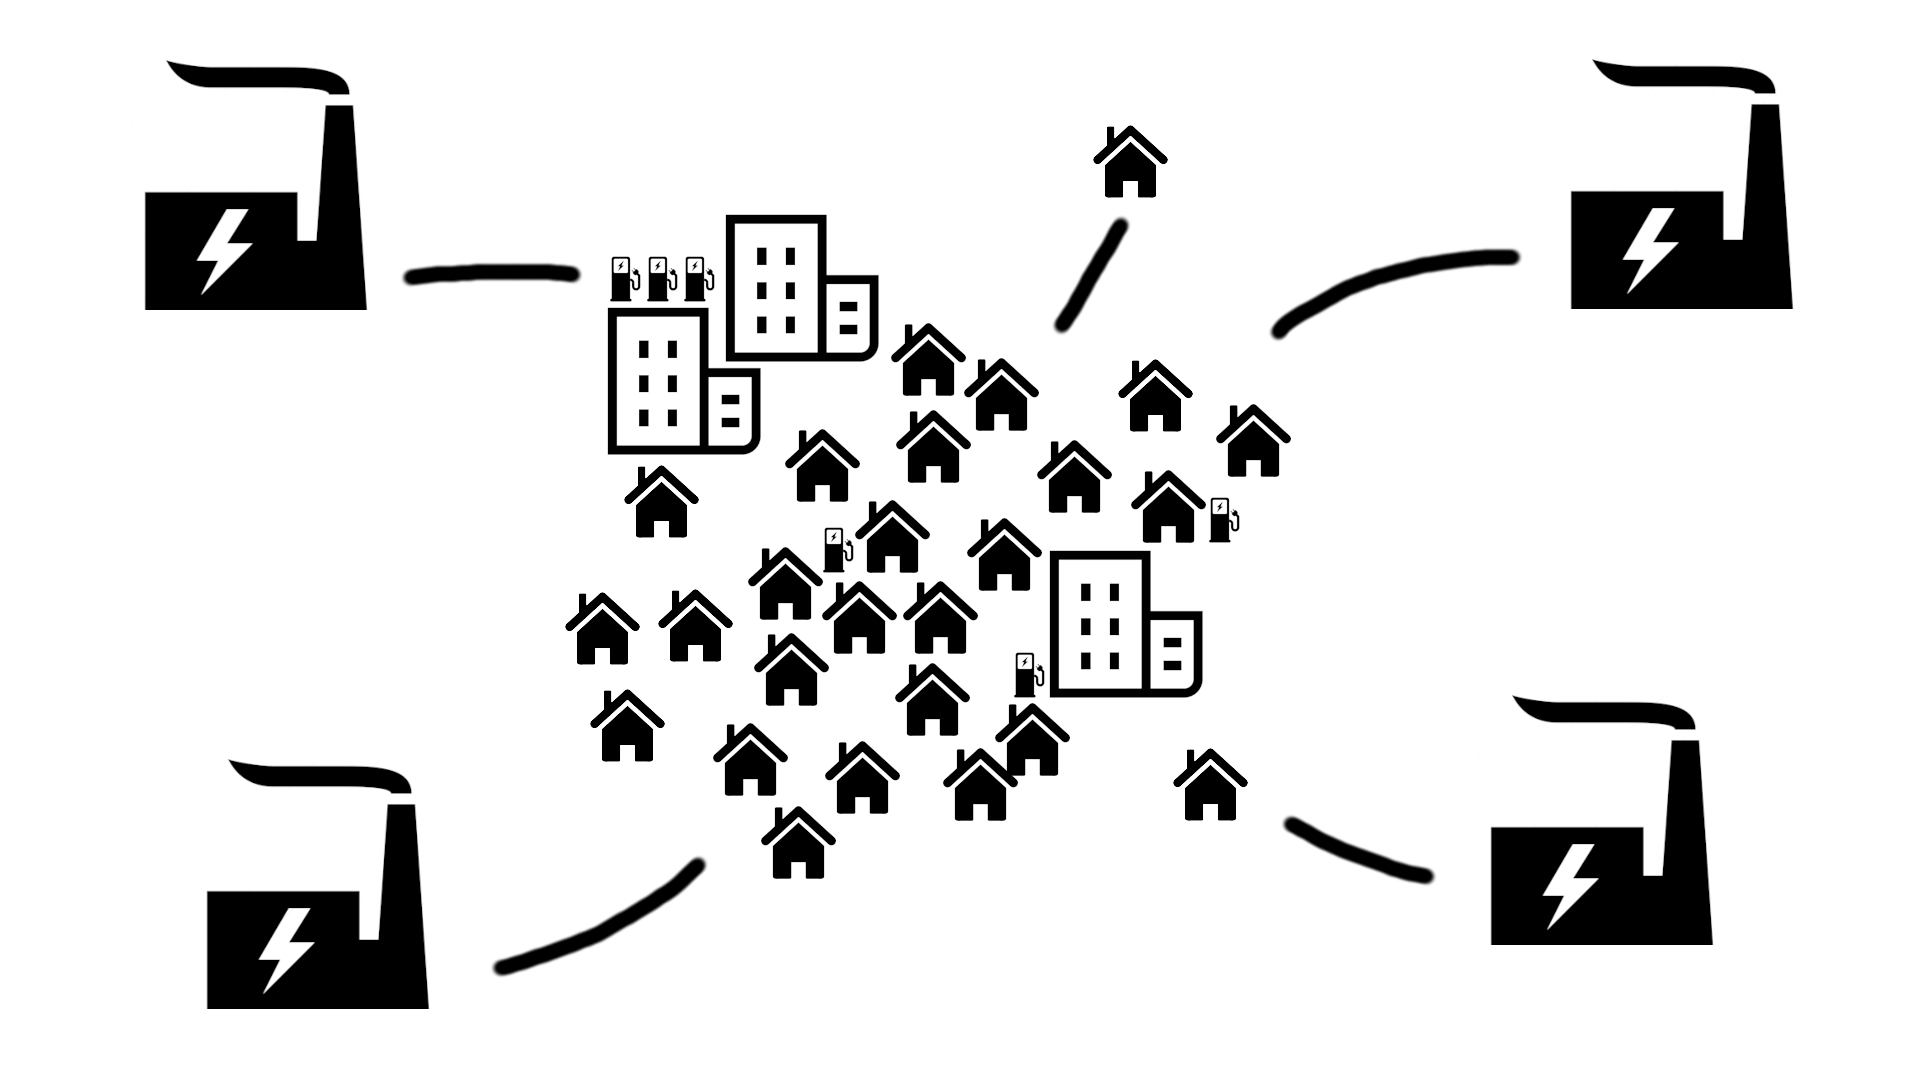
\includegraphics[width=\textwidth]{01_Intro/problem_sketch.png}
  \caption{Sketch of Unit Commitment Problem}
  \label{figure:problem.sketch}
\end{figure}

\chapter{Fundamentals}

\section{Unit Commitment Problem}
\label{fundamentals:ucp}

The Unit Commitment Problem (UCP) generally is concerned with the scheduling or ``commitment'' of thermal power plants over a given period.
Thermal power plants can be coal, oil, gas, or nuclear power plants.
The power plants should be scheduled such that the power demand or ``network load'' at each moment of the period is satisfied by the power output of the power plants.
While satisfying the demand, the sum of the fuel costs ($f_{i, t}$) should be minimal.
The fuel cost depends on the commitment of each power plant at each time ($u_{i, t}$), the power output of each power plant at each time ($p_{i, t}$), the power plant-specific cost function coefficients ($A_i$, $B_i$ and $C_i$), as well as start-up and shut-down costs ($A_{i}^{U}$ and $A_{i}^{D}$).
Other than the demand, the problem also considers various other constraints of the power plants.
These include the minimum and maximum power output of each plant ($P_{min, i}$ and $P_{max, i}$), the ramping constraints of each plant, and the minimum up and down-time~\cite{Baldick1995}.

This work only considers a subset of all possible constraints.
The demand, the minimum and maximum power output of the individual plant, and the startup and shutdown costs are considered.
So the goal is to minimize the sum of the cost functions ($f_{i, t}$) that also considers the startup and shutdown-costs.
Also, at each time instance, the combined power output satisfies the demand, and each power output does not violate the minimum and maximum power output of the power plant.

The UCP, this work considers, is non-linear because of the quadratic cost functions ($f_{i, t}$).
It also has floating-point variables and binary variables, where binary variables are represented as integer variables with domain $\{0, 1\}$.
The class of Mixed-Integer Non-Linear Problems (MINLP) is a class of optimization problems, with a non-linear objective function, integer and floating-point variables, and various constraints on the variables.
For that reason, the UCPs often are formulated as MINLPs.
These models are non-convex in the case of the UCP due to the binary nature of the commitment variables ($u_{i, t}$)~\cite{Baldick1995, Abujarad2017}.

\section{Mixed-Integer Non-linear Problems}
\label{fundamentals:minlp}

Mixed-integer Non-linear Problems (MINLPs) are a class of optimization problems that fit a specific form.
Formula (\ref{formula:minlp.form}) shows the from of MINLPs.
\begin{subequations}
  \label{formula:minlp.form}
  \begin{align}
    \min_x \quad
    & f(x)
    \label{formula:minlp.form.objective}
    \\
    s.t. \quad
    & g_j(x) \leq 0
    & \forall j \in M
    \label{formula:minlp.form.constraints}
    \\
    & x_i^l \leq x_i \leq x_i^u
    & \forall i \in N_0
    \label{formula:minlp.form.limits}
    \\
    & x_i \in \mathbb{Z}
    & \forall i \in N_0^I \subseteq N_0
    \label{formula:minlp.form.integer}
  \end{align}
\end{subequations}

where $f(x)$ and all $g(x)$ may be non-linear.
That is why the class of problems is called non-linear.

The first part (\ref{formula:minlp.form.objective}) is the objective function.
The goal is to find an input $x \in \mathbb{R}^n$ that minimizes $f(x)$ while also respecting the constraints.
The second part (\ref{formula:minlp.form.constraints}) lists all the constraints that involve multiple elements of the input x.
The input $x$ has to comply with all constraints.
The third part (\ref{formula:minlp.form.limits}) sets limits for the elements $x_i$ of $x$.
And the last part \ref{formula:minlp.form.integer} states that some of the elements $x_i$ are integers rather than rational numbers~\cite{Belotti2009}.

Optimizing MINLPs is NP-complete~\cite{Bienstock1996}.
That means that no known algorithm can optimize all possible MINLPs with polynomial time complexity.

\section{Quantum Computing}

Quantum computers use quantum bits (qubits) instead of normal bits that classical computers use.
While a bit can be either in the state $0$ or $1$, a qubit can be in a so-called superposition of two states.
States of qubits are generally written using the Dirac-Notation, also known as the Bra-Ket-Notation
The two states, the superposition is a combination of, are called the basis.
The most basic basis is the basis $\{ \ket{0}, \ket{1} \}$.
The formula (\ref{formula:quantum.superposition}) describes such a superposition.
When one measures the state of the qubit, it collapses into one of the base states, which is the result of the measurement.
The probability of either basis state being measured is the square of the the complex amplitude of the basis state in the superposition.
\cite{Vedral1998}
\begin{subequations}
\begin{align}
  \label{formula:quantum.superposition}
  & \ket{\phi} = \alpha \cdot \ket{0} + \beta \cdot \ket{1}
  & \text{with } \alpha, \beta \in \mathbb{C}, \alpha^2 + \beta^2 = 1
  \\
  & P(\ket{0}) = \alpha^2
\end{align}
\end{subequations}

\input{02_Background/03_Quantum/01_annealing}
\input{02_Background/03_Quantum/02_gatebased}

\section{Related Work}

\subsection{Unit Commitment Problem}

Many methods for optimizing the UCP described in section \ref{backg:ucp} exist in the literature.
Abujarad et al. \cite{Abujarad2017} listed and compared those methods.
They listed the use of Mixed-integer Linear Programming as accurate but exponentially expensive.
All other methods give a sub-optimal solution.
\cite{Abujarad2017}

When dealing with cost functions of thermal power plants, they seldom are linear.
Most commonly, they are quadratic.
Baldick \cite{Baldick1995} generalized the formulation of the UCP as Mixed-integer Non-linear Problems, where he assumed a quadratic cost function.

\subsection{Quantum Computing for Unit Commitment}

Ajagekar and You \cite{Ajagekar2019} explore the utility of quantum computing for optimization problems in the energy domain.
They also considered the UCP.
They formulated a UCP as a QUBO and used D-Wave quantum hardware (the D-Wave 2000Q, to be precise) to optimize that model of the UCP.
Compared to the optimization on a classical computer using the Gurobi solver, the quantum option did perform terribly.
\cite{Ajagekar2019}

\subsection{Discrete Quadratic Model Optimization on Quantum Computers}


\chapter{Approach}

\section{Unit Commitment Problem as Mixed-Integer Nonlinear Problem}

The UCP is formulated as a MINLP for classical computers to solve,
as mentioned in section \ref{fundamentals:ucp}.
The equations (\ref{formula:minlp}) represent the formulated MINLP.

\begin{subequations}
\begin{align}
  \min_{u, p} \quad &
  \sum_{i \in \mathbb{I}, t \in \mathbb{T}} f_{i, t}
  = \sum_{i \in \mathbb{I}, t \in \mathbb{T}}
    u_{i, t} (A_i + B_i p_{i, t}' + C_i (p_{i, t}')^2) + s_{i, t}
  \label{formula:minlp.obj} \\
  \text{s.t.} \quad & l_t = \sum_{i \in \mathbb{I}} u_{i, t} p_{i, t}' \quad &
  \forall t \in \mathbb{T}
  \label{formula:minlp.load} \\
  &
  P_{min, i} \leq p_{i, t}' \leq P_{max, i} \quad &
  \forall i \in \mathbb{I}, t \in \mathbb{T}
  \label{formula:minlp.power} \\
  &
  s_{i, t} = \begin{cases}
    A_i^U & \text{if } u_{i, t} > u_{i, t-1} \\
    A_i^D & \text{if } u_{i, t} < u_{u, t-1} \\
    0 & \text{else}
  \end{cases} \quad &
  \forall i \in \mathbb{I}, t \in \mathbb{T}
  \label{formula:minlp.updowncost}
\end{align}
\label{formula:minlp}
\end{subequations}

\subsubsection{Objective Function}

The formula (\ref{formula:minlp.obj}) represents the global cost function.
This function has to be minimized and is called the ''objective function''.
It is the sum of all cost functions $f_{i, t}$ of the individual power plants at every time step.

The individual cost funtions $f_{i, t}$ take $u_{i, t}$ and $p_{i, t}'$ as free variables.
$A_i, B_i$ and $C_i$ are constant for every power plant.
$f_{i, t}$ also depend on $s_{i, t}$ or equation (\ref{formula:minlp.updowncost}),
which evaluates to $A_i^U, A_i^D$ or $0$ depending on the free commitment variables $u_{i, t}$ and $u_{i, t-1}$.
$A_i^U$ and $A_i^D$ are also constant for every power plant,
as well as $u_{i, -1}$.

$A_i, A_i^U$ and $A_i^D$ are the linear coefficients of the cost function,
because they are not a factor of $p_{i, t}$.
$A_i$ is the constant cost when the power plant is active
and is added to $f_{i, t}$ if $u_{i, t} = 1$.
$A_i^U$ is the cost of starting the power plant
and is added to $f_{i, t}$ if $u_{i, t} > u_{i, t-1}$.
$A_i^D$ is the cost of shutting down the power plant
and is added to $f_{i, t}$ if $u_{i, t} < u_{i, t-1}$.
If $t = 0$ this would lead to problems, because $u_{i, t-1} = u_{i, -1}$ would be undefined.
That's why the initial state of the power plant $u_{i, -1}$ is also constant.
$B_i$ is the linear coefficient of the cost function,
because it is a factor of $p_{i, t}'$.
It is multiplied by $p_{i, t}'$ and added to $f_{i, t}$ if $u_{i,  t} = 1$.
$C_i$ is the quadratic coefficient of the cost function,
because it is a factor of $p_{i, t}^2$.
It is multiplied by $p_{i, t}^2$ and added to $f_{i, t}$ if $u_{i,  t} = 1$.

So the obbjective function takes the free variables
$
(u_{i, t})_{i \in \mathbb{I}, t \in \mathbb{T}},
(p_{i, t}')_{i \in \mathbb{I}, t \in \mathbb{T}}
$ and the constants $
(A_i)_{i \in \mathbb{I}},
(A_i^U)_{i \in \mathbb{I}},
(A_i^D)_{i \in \mathbb{I}},
(B_i)_{i \in \mathbb{I}},
(C_i)_{i \in \mathbb{I}},
$ and $
(u_{i, -1})_{i \in \mathbb{I}}
$ as input.
The free variables are chosen, such that the objective function is minimized.

\subsubsection{Constraints}

As the optimal inputs are computed, the optimizer has to also take the constraints into account.
These are given as equations or inequations.
In this case there is one equation (\ref{formula:minlp.load}) and one inequation (\ref{formula:minlp.power}).

The equation (\ref{formula:minlp.load}) makes sure, that the combined power
of all power plants equals the power demand or ''load'' at each time instance $t$.
This is achieved by setting each constant $(l_t)_{t \in \mathbb{T}}$
equal to the sum of the power of all power plants at that time $t$.
The summands on the right-hand side are the multiplication of
$u_{i, t}$ and $p_{i, t}'$ and not simply $p_{i, t}'$,
because in this model the power output can be greater than 0
when the unit is not committet.
This is a modeling trick, in order to enable the modeling of the inequation (\ref{formula:minlp.power}).

The inequation (\ref{formula:minlp.power}) makes sure, that the power output $p_{i, t}'$
of each power plant $i$ at each time intance $t$ is within the limits of the power plant.
These limits are $P_{min, i}$ for the minimum and $P_{max, i}$ for the maximum
power output.
As mentioned earlier, the power output $p_{i, t}'$ never reaches 0,
if $P_{min, i}$ is greater than 0.
So after finding the minimum inputs $u$ and $p'$ for the MINLP problem,
the solution to the UCP is the actual power $p_{i, t} = u_{i, t} p_{i, t}'$.

\section{Performance of Classical Computers}

For the optimization of the Pyomo model, the Pyomo library runs a standard solver.
It formulates the problem in the mathematical modeling language AMPL
and calls a solver to optimize it.
The solver returns the solution, which Pyomo then reads~\cite{PyomoAMPL}.

This work uses the open-source solver Couenne for classical optimizations.
COIN-OR built this solver.
Couenne is short for ``Convex Over and Under ENvelopes for Nonlinear Estimation''.
It can find global minima of nonconvex MINLPs like the one that this work considers.
It is a branch and bound algorithm and utilizes linearization, bound reduction, and branching methods~\cite{Belotti2009, CoinorHome, CouenneRepo}.

This work performs the classical optimizations on the Excess Cluster of the HLRS, Stuttgart~\cite{ExcessHLRS, HLRS}.

The optimization of the problem is of high time complexity.
In the beginning, with small inputs, it takes little time.
As listed in table \ref{table:evaluation.classical.performance}, the optimization of $4$ power plants with $2$ units of time takes about $0.5$ seconds.
But as the input size grows, the time needed by the solver grows exponentially.
When the input size is doubled --- $4$ plants over $4$ units of time --- the optimization takes about $3.5$ seconds.
After adding another $2$ units of time, the optimization takes $15.5$ seconds.

As the number of inputs grows large, the optimization grows even faster than exponentially.
With a worst-case projection of the first $4$ data points, the time needed for optimization should multiply by $7$ with every additional $2$ units of time.
That means that the optimization of $4$ power plants over $14$ units of time should take about $0.5 \cdot 7^6 \approx 58,824$ seconds.
But the data shows that it took about $311,144.9$ seconds.

\begin{table}[ht]
  \centering
  \input{81_Tables/04_Validation/performance_classical_p4}
  \caption{Results of Classical Optimization with $4$ Power Plants}
  \label{table:evaluation.classical.performance}
\end{table}

The diagram \ref{figure:evaluation.classical.performance} highlights the fast growing computation time needed for the optimization.
Only the last two data points are distinguishable from the first data points because their computation time is very long compared to the first data points.
It shows the time needed for optimization dependent on the input size --- the number of time instances.

\begin{figure}[ht]
  \centering
  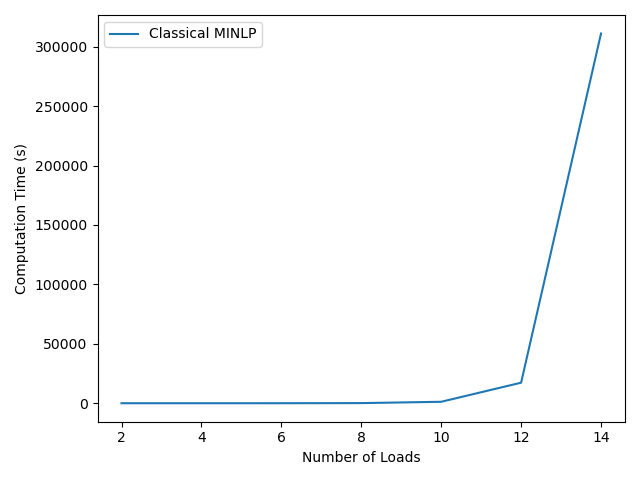
\includegraphics[width=0.75 \textwidth]{04_Validation/performance_classical_p4.png}
  \caption{Time Complexity of Classical Optimization with $4$ Power Plants}
  \label{figure:evaluation.classical.performance}
\end{figure}

\section{Performance of Annealing-based Quantum Computers}

\subsection{Hybrid DQM Solver}

For the optimization using the Quantum Annealing hardware, the formulated DQM is sent to a hybrid solver at D-Wave.
The hybrid solver does not put the DQM on quantum hardware directly.
It classically searches the solution space.
The hybrid solver speeds up this process by using quantum hardware to determine promising regions to explore next.
\cite{DQMHybrid2020}

The optimization of the DQM using the hybrid solver for small problems seems to have linear time complexity.
Every time $10$ time instances are added to the problem size, the optimization takes about $0.1$ seconds longer.
The results of the optimization and the time needed for the optimization are listed in table \ref{table:validation.annealing.performance}.
The optimization of these problems takes no longer than $5.6$ seconds each.

\begin{table}[ht]
  \centering
  \input{81_Tables/04_Validation/performance_annealing_p4.tex}
  \caption{Results of Annealing Optimization with $4$ Power Plants}
  \label{table:validation.annealing.performance}
\end{table}

In figure \ref{figure:validation.annealing.performance} the time complexity is displayed clearer.
The time needed for optimizing problems with less than $15$ time instances also seems to be constant.
After that, the linear time complexity is clearly visible.

When the problem size increases, the time complexity seems to be worse than linear.
This becomes clear in figure \ref{figure:validation.annealin.performance.extended}.
The time taken by the hybrid solver to optimize the problem grows linearly, but at a higher rate starting from $80$ time instances.
After this increase of slope, the slope stays the same until the problem size reaches $200$ in the time dimension.
I did not test the optimization of problems with more than $200$ time instances on the D-Wave hardware.

\begin{figure}
  \begin{subfigure}[b]{0.5 \textwidth}
    \centering
    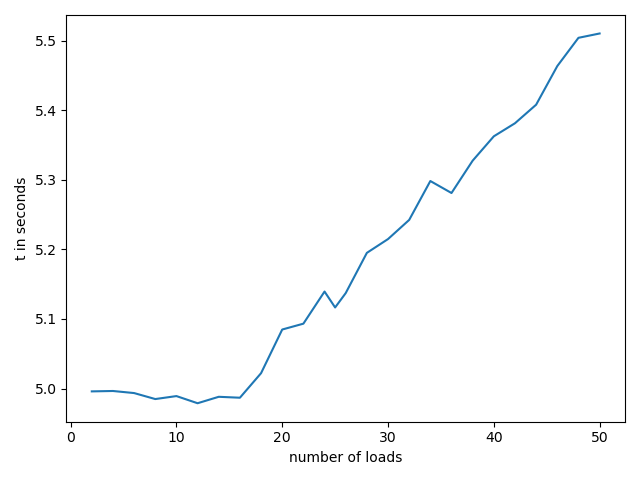
\includegraphics[width=\textwidth]{04_Validation/performance_annealing_p4.png}
    \caption{With up to $50$ Loads}
    \label{figure:validation.annealing.performance}
  \end{subfigure}
  \begin{subfigure}[b]{0.5 \textwidth}
    \centering
    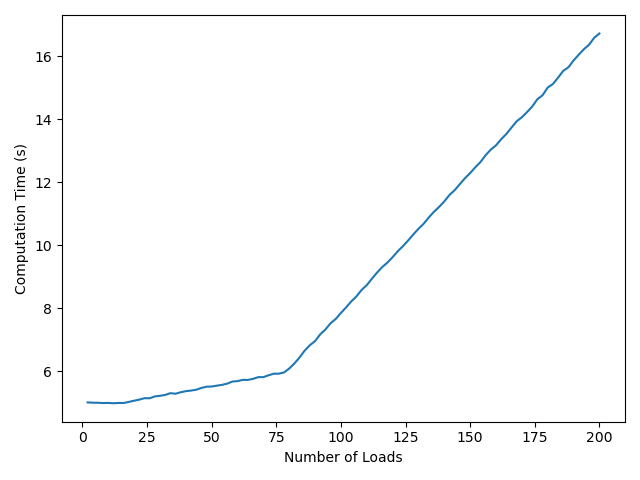
\includegraphics[width=\textwidth]{04_Validation/performance_annealing_p4_extended.png}
    \caption{With up to $200$ Loads}
    \label{figure:validation.annealin.performance.extended}
  \end{subfigure}
  \caption{Time Complexity of Annealing Optimization with $4$ Power Plants}
\end{figure}

This approach does not produce optimal solutions for the UCP.
The summed power output of the single power plants does not meet the power demand because the DQM underestimates the demand part of the UCP.
After retrieving the optimal DQM solution and translating it to a UCP solution, the program adjusts the power outputs of the power plants.
It does so as described in section \ref{approach:quantum.read.solution}.
This leads to a non-optimal solution of the UCP.

\subsubsection{Hybrid QUBO Solver}

\todo{list results of hybrid QUBO solver}

\subsubsection{Direct QUBO Solver}

D-Wave's QPUs can embed many QUBOs on them.
But if a QUBO has too many variables or quadratic biases connecting the biases, D-Wave might not find an embedding.
That is the case for the problems this work considers.

The smallest problem formulated as a QUBO has $1, 024$ variables and $263, 680$ quadratic biases.
These values can be calculated using formulas (\ref{formula:qubo.num.variables}) and (\ref{formula:qubo.num.quadratic.biases}) respectively.
One variable can have more than $255$ quadratic biases.
The reason is that power plant $4$ has $2^8$ possible power levels after discretizing the power levels, and variables for the different power levels of one power plant at one time instances are connected with quadratic biases.

Since the ''Advantage'' QPU has a $15$-way qubit connectivity, it would need an enormous amount of physical qubits to represent one logical binary variable.
More as there are available on the ''Advantage'' QPU.
\cite{D-Wave2020, Zbinden2020}
Because of this, the minor miner can't find embeddings for the QUBOs this work considers.
An algorithm designed specifially for embedding large cliques by \citeauthor{Zbinden2020}, can not embed cliques larger than $180$ for the ''Pegasus'' architecture.
\cite{Zbinden2020}

\section{Performance of Gate-based Quantum Computers}

The implementation of the QUBO as described in section \ref{approach:gate.implement} of the UCP builds a quantum circuit for the first iteration of the optimization algorithm described in section \ref{backg:quantum.grover.optimization}.
Unfortunately, this quantum circuit is too big to be executed on any of IBM's public quantum computers for the smallest UCP that this work considers.

The number of qubits needed just for the QUBO variables is the same as the number of binary variables in the QUBO.
The number of variables in a QUBO is given by the formula (\ref{formula:qubo.num.variables}).
These qubits are considered the first quantum register of the quantum circuit.
In the case of the smallest UCP, this work considers with the $4$ power plants listed in section \ref{table:validation.data.plants} and $2$ time instances, the number of qubits would be $1, 024$.
With every additional $2$ time instances of the UCP, the algorithm needs another $1, 024$ qubits.

Additionally to this quantum register, the algorithm needs a second quantum register for storing the result of the QUBO dependent on the QUBO variables of the first register.
The domain of values the QUBO produces grows with the size of the QUBO.
It is proportional to the number of biases assuming the average value of the biases stays the same.

Regardless of the number of gates the quantum circuit would have, the gate-based quantum computers right now do not have enough qubits to handle the problems this work considers.


\chapter{Implementation}

\section{Performance of Classical Computers}

For the optimization of the Pyomo model, the Pyomo library runs a standard solver.
It formulates the problem in the mathematical modeling language AMPL
and calls a solver to optimize it.
The solver returns the solution which is then read by Pyomo.
\cite{PyomoAMPL}

The solver that is used in this paper is called Couenne and was built by COIN-OR.
Couenne is short for ''Convex Over and Under ENvelopes for Nonlinear Estimation''.
It can find global minima of nonconvex MINLPs like the one that is formulated above.
It is a branch and bound algorithm and utilizes linearization, bound reduction, and branching methods.
\cite{CoinorHome,CouenneRepo}

The optimizations are performed on the Excess Cluster of the HLRS, Stuttgart.
\cite{ExcessHLRS,HLRS}

The optimization of the problem has a really high time complexity.
In the beginning with small inputs, it is very fast.
As listed in table \ref{table:validation.classical.performance}, the optimization of 4 power plants with 2 units of time takes about 0.5 seconds.
But as the input size grows, the time needed by the solver grows exponentially.
When the input size is doubled --- 4 plants over 4 time units --- the optimization takes about 3.5 seconds.
Adding another 2 time units, the optimization the takes 15.5 seconds.

As the number of inputs grow even larger, the optimization grows even faster than exponentially.
With a worst-case projection of the forst 4 data points, the time needed for optimization should multiply by 7 with every additional 2 units of time.
That means, that the optimization of 4 power plants over 14 units of time should take about $0.5s \cdot 7^6 \approx 58,824s$.
But the data shows that it took about $311,144.9$ seconds.

\begin{table}[ht]
  \centering
  \input{81_Tables/04_Validation/performance_classical_p4}
  \caption{Results of classical optimization with four power plants.}
  \label{table:validation.classical.performance}
\end{table}

\begin{figure}[ht]
  \centering
  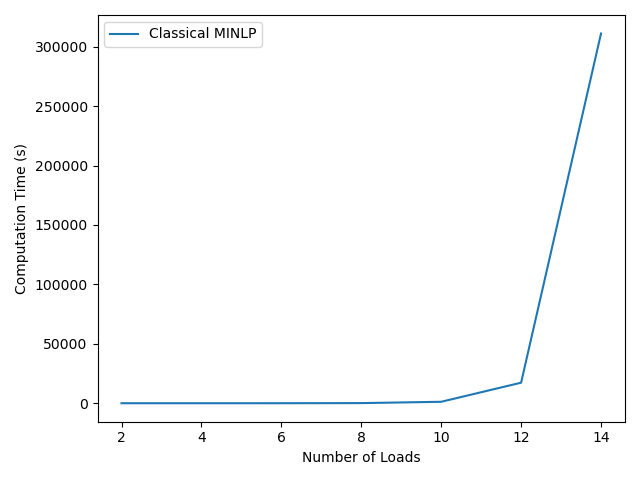
\includegraphics[width=0.75 \textwidth]{04_Validation/performance_classical_p4.png}
  \caption{Time complexity of classical optimization with four power plants.}
  \label{figure:validation.classical.performance}
\end{figure}

\input{03_Approach/01_Annealing/01_dqm}
\input{03_Approach/01_Annealing/02_annealing_implementation}

\section{Implementation for Gate-based Quantum Computers}
\label{implement:gate.qubo}

The implementation for the gate-based quantum computers uses the Qiskit framework.
Qiskit is an open-source framework for quantum computing on gate-based quantum computers.
It was founded by IBM Research.
\cite{QiskitWeb, QiskitGitHub}
After the program instantiates the QUBO using the \texttt{QuadraticProgram} class of the framework, it uses the class \texttt{GroverOptimizer} to optimize the QUBO.
This class handles building the quantum circuits and executing the computation for the Grover Optimization algorithm as described in section \ref{fundamentals:quantum.grover.optimization}.

\subsubsection{Variables}

In this implementation, the variables are not implicit as with the UQO-client in section \ref{implementation:annealing.qubo.variables}.
The program instantiates all binary variables of the QUBO at the beginning of building the QUBO instance.
It assigns a name to every variable that holds the indices of the corresponding power plant $i$, time instance $t$, and power output level $k$.

\subsubsection{Quadratic Biases}

The program adds the same quadratic biases as the implementation for annealing quantum computers in section \ref{implementation:annealing.qubo.quadratic}.
It stores the biases in a python \texttt{dict} with keys that are pairs of strings.
The strings are the names of the variables.

\subsubsection{Linear Biases}

The program adds the same linear biases as the implementation for annealing quantum computers in section \ref{implementation:annealing.qubo.linear}.
It stores the biases in a python \texttt{dict} with keys that are strings.
The strings are again the names of the variables.

\subsubsection{Canstant Bias}

As mentioned before in section \ref{implementation:annealing.qubo.constant}, the constant bias does not change the input that produces a optimum of the QUBO.
But with this framework, the interface allows for a constant bias to be added to the QUBO.
The implementation computes the bias once, as specified in the formula (\ref{formula:qubo.result.constant}, and adds it to the QUBO instance.

\section{Converting Solutions of Quadratic Models}

\subsection{Choosing Power Levels}
\label{implementation:quantum.read.solution.qubo}

For QUBOs, it can happen that for a single power plant at a single time instance, multiple binary variables for different power levels are $1$.
The program then has to choose one of the possible power levels where the binary variable is $1$.
For this the algorithm \ref{implementation:quantum.read.solution.qubo.algorithm} is used.

\begin{lstlisting}[
  caption={Choosing Power Levels from the QUBO},
  label={implementation:quantum.read.solution.qubo.algorithm},
  language=Python
]
value_indices: List[int] = []
for k in range(len(self.P[i])):
  if result[self.p[i][t][k].name] == 1:
    value_indices.append(k)

value: float = 0
num_indices: int = len(value_indices)
if num_indices > 0:
  value = self.P[i][value_indices[(int) (num_indices / 2)]]
  if num_indices > 1:
    debug_msg('Warning: {} possible power levels for plant {} detected'.format(num_indices, i))
\end{lstlisting}

The program always chooses the median value.

\subsection{Adjusting Power Levels}
\label{implementation:quantum.read.solution}

The program translates the optimal solution of the DQM or QUBO to a solution for the UCP.
This solution, however, is not legal.
The sum of the power outputs at every time instance does not satisfy the demand.
The program, therefore, raises the power outputs of all plants at every time instance uniformly.
While doing so, it also avoids violating the power limits of the individual plants.
For this the algortihm \ref{implementation:quantum.read.solution.algorithm} is used.

\begin{lstlisting}[
  caption={Adjusting the UCP Solution},
  label={implementation:quantum.read.solution.algorithm},
  language=Python
]
for t in range(self.ucp.parameters.num_loads):
  adjust: List[bool] = [u[i][t] for i in range(self.ucp.parameters.num_plants)]
  delta: float = self.ucp.loads[t] - sum([p[i][t] for i in range(self.ucp.parameters.num_plants)])

  while True:
    if delta == 0 or not functools.reduce(lambda a,b: a or b, adjust):
      break

    adjustment: float = delta / sum([1 if b else 0 for b in adjust])
    delta = 0

    for i in range(self.ucp.parameters.num_plants):
      if adjust[i]:
        p[i][t] += adjustment
        Pmax: float = self.ucp.plants[i].Pmax
        Pmin: float = self.ucp.plants[i].Pmin

        if p[i][t] > Pmax:
          delta += p[i][t] - Pmax
          p[i][t] = Pmax
          adjust[i] = False

        elif p[i][t] < Pmin:
          delta += p[i][t] - Pmin
          p[i][t] = Pmin
          adjust[i] = False
\end{lstlisting}


\chapter{Evaluation}
\label{evaluation}

\section{Data used for Validation}
\label{validation:data}

\subsection{Consumers}

This work considers real-world demand data of energy consumers.
It takes the data from two different sources.
\begin{enumerate*}
  \item Smart meters that Georgievski \citeauthor{Georgievski2012} installed in an office. \cite{Georgievski2012}
  \item Adaptive Charging Network (ACN) electric vehicle charging stations at the Californian Institute of Technology. \cite{Lee2019, ACNCaltech2020}
\end{enumerate*}

The data from the smart meters spans about $8$ months.
It is from the year 2016.
It has a time resolution of $10$ seconds.
The program transforms the data to have a time resolution of $10$ minutes.
It does so by adding up the energy demand of $10$ minute periods and then dividing by $0.166$ hours since the data is given as energy in kWh.
The result is the power given in kW.

The data from the ACN charging stations spans the first $9$ months of the year 2020.
It consists of various charging sessions.
The program identifies the energy demand by assuming the charger transfers energy to the car at one fixed rate in one session.
This is not the point of adaptive charging, but it gives a real-world-like representation of electric vehicle charging behavior.
The time resolution of the resulting data is $10$ minutes.

The program computes the average day of both datasets.
Then it combines both datasets.
The data from the smart meters is weighted $1, 000 : 1$ against the data from the ACN charging stations.
This composition is due to the low energy demand of one office.
The final data represents an average day of one electric vehicle charging site and $1, 000$ offices with a $10$ minute time resolution.
It is shown in figure \ref{figure:data.demand.day}.

\begin{figure}
  \centering
  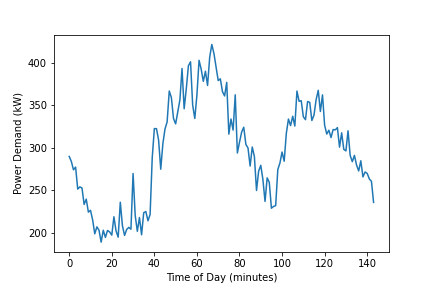
\includegraphics[width=0.7 \textwidth]{04_Validation/data_demand_day.png}
  \caption{Demand Data}
  \label{figure:data.demand.day}
\end{figure}

\subsection{Producers}

\todo{List data of plants}

\section{Performance of Classical Computers}

For the optimization of the Pyomo model, the Pyomo library runs a standard solver.
It formulates the problem in the mathematical modeling language AMPL
and calls a solver to optimize it.
The solver returns the solution, which Pyomo then reads~\cite{PyomoAMPL}.

This work uses the open-source solver Couenne for classical optimizations.
COIN-OR built this solver.
Couenne is short for ``Convex Over and Under ENvelopes for Nonlinear Estimation''.
It can find global minima of nonconvex MINLPs like the one that this work considers.
It is a branch and bound algorithm and utilizes linearization, bound reduction, and branching methods~\cite{Belotti2009, CoinorHome, CouenneRepo}.

This work performs the classical optimizations on the Excess Cluster of the HLRS, Stuttgart~\cite{ExcessHLRS, HLRS}.

The optimization of the problem is of high time complexity.
In the beginning, with small inputs, it takes little time.
As listed in table \ref{table:evaluation.classical.performance}, the optimization of $4$ power plants with $2$ units of time takes about $0.5$ seconds.
But as the input size grows, the time needed by the solver grows exponentially.
When the input size is doubled --- $4$ plants over $4$ units of time --- the optimization takes about $3.5$ seconds.
After adding another $2$ units of time, the optimization takes $15.5$ seconds.

As the number of inputs grows large, the optimization grows even faster than exponentially.
With a worst-case projection of the first $4$ data points, the time needed for optimization should multiply by $7$ with every additional $2$ units of time.
That means that the optimization of $4$ power plants over $14$ units of time should take about $0.5 \cdot 7^6 \approx 58,824$ seconds.
But the data shows that it took about $311,144.9$ seconds.

\begin{table}[ht]
  \centering
  \input{81_Tables/04_Validation/performance_classical_p4}
  \caption{Results of Classical Optimization with $4$ Power Plants}
  \label{table:evaluation.classical.performance}
\end{table}

The diagram \ref{figure:evaluation.classical.performance} highlights the fast growing computation time needed for the optimization.
Only the last two data points are distinguishable from the first data points because their computation time is very long compared to the first data points.
It shows the time needed for optimization dependent on the input size --- the number of time instances.

\begin{figure}[ht]
  \centering
  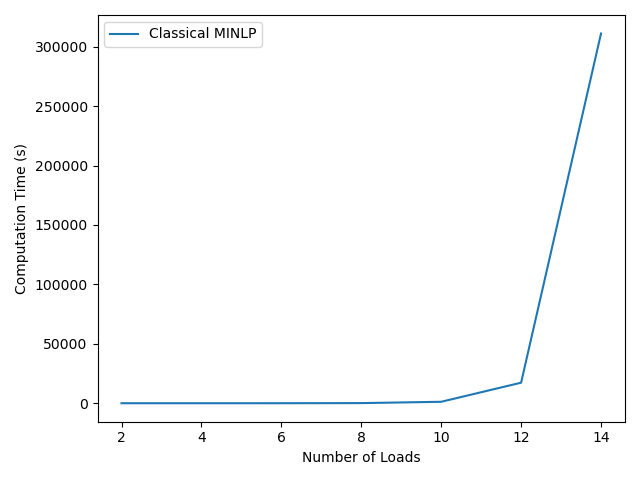
\includegraphics[width=0.75 \textwidth]{04_Validation/performance_classical_p4.png}
  \caption{Time Complexity of Classical Optimization with $4$ Power Plants}
  \label{figure:evaluation.classical.performance}
\end{figure}

\section{Performance of Annealing-based Quantum Computers}

\subsection{Hybrid DQM Solver}

For the optimization using the Quantum Annealing hardware, the formulated DQM is sent to a hybrid solver at D-Wave.
The hybrid solver does not put the DQM on quantum hardware directly.
It classically searches the solution space.
The hybrid solver speeds up this process by using quantum hardware to determine promising regions to explore next.
\cite{DQMHybrid2020}

The optimization of the DQM using the hybrid solver for small problems seems to have linear time complexity.
Every time $10$ time instances are added to the problem size, the optimization takes about $0.1$ seconds longer.
The results of the optimization and the time needed for the optimization are listed in table \ref{table:validation.annealing.performance}.
The optimization of these problems takes no longer than $5.6$ seconds each.

\begin{table}[ht]
  \centering
  \input{81_Tables/04_Validation/performance_annealing_p4.tex}
  \caption{Results of Annealing Optimization with $4$ Power Plants}
  \label{table:validation.annealing.performance}
\end{table}

In figure \ref{figure:validation.annealing.performance} the time complexity is displayed clearer.
The time needed for optimizing problems with less than $15$ time instances also seems to be constant.
After that, the linear time complexity is clearly visible.

When the problem size increases, the time complexity seems to be worse than linear.
This becomes clear in figure \ref{figure:validation.annealin.performance.extended}.
The time taken by the hybrid solver to optimize the problem grows linearly, but at a higher rate starting from $80$ time instances.
After this increase of slope, the slope stays the same until the problem size reaches $200$ in the time dimension.
I did not test the optimization of problems with more than $200$ time instances on the D-Wave hardware.

\begin{figure}
  \begin{subfigure}[b]{0.5 \textwidth}
    \centering
    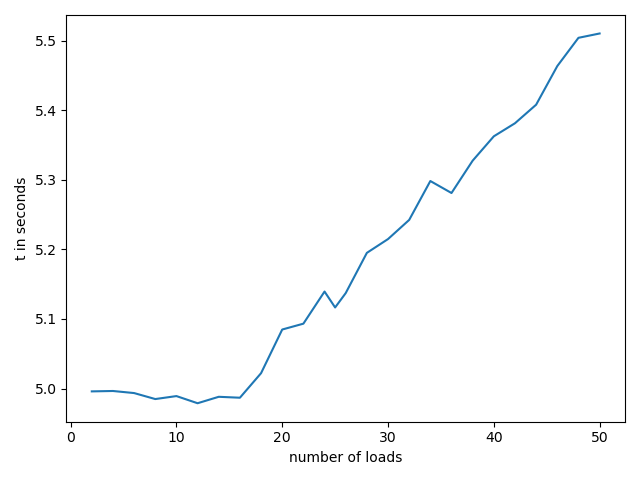
\includegraphics[width=\textwidth]{04_Validation/performance_annealing_p4.png}
    \caption{With up to $50$ Loads}
    \label{figure:validation.annealing.performance}
  \end{subfigure}
  \begin{subfigure}[b]{0.5 \textwidth}
    \centering
    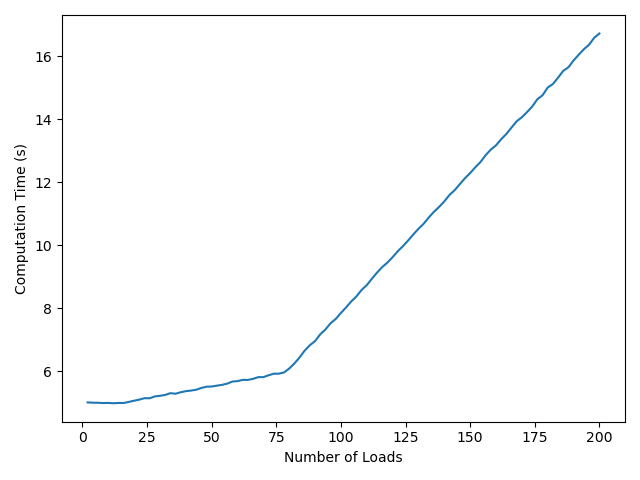
\includegraphics[width=\textwidth]{04_Validation/performance_annealing_p4_extended.png}
    \caption{With up to $200$ Loads}
    \label{figure:validation.annealin.performance.extended}
  \end{subfigure}
  \caption{Time Complexity of Annealing Optimization with $4$ Power Plants}
\end{figure}

This approach does not produce optimal solutions for the UCP.
The summed power output of the single power plants does not meet the power demand because the DQM underestimates the demand part of the UCP.
After retrieving the optimal DQM solution and translating it to a UCP solution, the program adjusts the power outputs of the power plants.
It does so as described in section \ref{approach:quantum.read.solution}.
This leads to a non-optimal solution of the UCP.

\subsubsection{Hybrid QUBO Solver}

\todo{list results of hybrid QUBO solver}

\subsubsection{Direct QUBO Solver}

D-Wave's QPUs can embed many QUBOs on them.
But if a QUBO has too many variables or quadratic biases connecting the biases, D-Wave might not find an embedding.
That is the case for the problems this work considers.

The smallest problem formulated as a QUBO has $1, 024$ variables and $263, 680$ quadratic biases.
These values can be calculated using formulas (\ref{formula:qubo.num.variables}) and (\ref{formula:qubo.num.quadratic.biases}) respectively.
One variable can have more than $255$ quadratic biases.
The reason is that power plant $4$ has $2^8$ possible power levels after discretizing the power levels, and variables for the different power levels of one power plant at one time instances are connected with quadratic biases.

Since the ''Advantage'' QPU has a $15$-way qubit connectivity, it would need an enormous amount of physical qubits to represent one logical binary variable.
More as there are available on the ''Advantage'' QPU.
\cite{D-Wave2020, Zbinden2020}
Because of this, the minor miner can't find embeddings for the QUBOs this work considers.
An algorithm designed specifially for embedding large cliques by \citeauthor{Zbinden2020}, can not embed cliques larger than $180$ for the ''Pegasus'' architecture.
\cite{Zbinden2020}

\section{Performance of Gate-based Quantum Computers}

The implementation of the QUBO as described in section \ref{approach:gate.implement} of the UCP builds a quantum circuit for the first iteration of the optimization algorithm described in section \ref{backg:quantum.grover.optimization}.
Unfortunately, this quantum circuit is too big to be executed on any of IBM's public quantum computers for the smallest UCP that this work considers.

The number of qubits needed just for the QUBO variables is the same as the number of binary variables in the QUBO.
The number of variables in a QUBO is given by the formula (\ref{formula:qubo.num.variables}).
These qubits are considered the first quantum register of the quantum circuit.
In the case of the smallest UCP, this work considers with the $4$ power plants listed in section \ref{table:validation.data.plants} and $2$ time instances, the number of qubits would be $1, 024$.
With every additional $2$ time instances of the UCP, the algorithm needs another $1, 024$ qubits.

Additionally to this quantum register, the algorithm needs a second quantum register for storing the result of the QUBO dependent on the QUBO variables of the first register.
The domain of values the QUBO produces grows with the size of the QUBO.
It is proportional to the number of biases assuming the average value of the biases stays the same.

Regardless of the number of gates the quantum circuit would have, the gate-based quantum computers right now do not have enough qubits to handle the problems this work considers.

\section{Comparison of Performances}
\label{validation:comparison}

\todo{Compare performances of classical, annealing-based and gate-based Computers}

\begin{figure}
  \begin{subfigure}[b]{0.5 \textwidth}
    \centering
    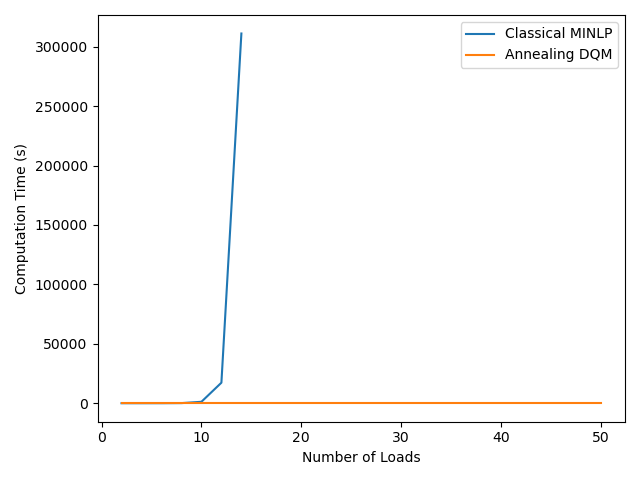
\includegraphics[width=\textwidth]{04_Validation/comparison_performance_c_dqm_p4.png}
    \caption{With up to $50$ Loads}
    \label{figure:validation.performance.comparison}
  \end{subfigure}
  \begin{subfigure}[b]{0.5 \textwidth}
    \centering
    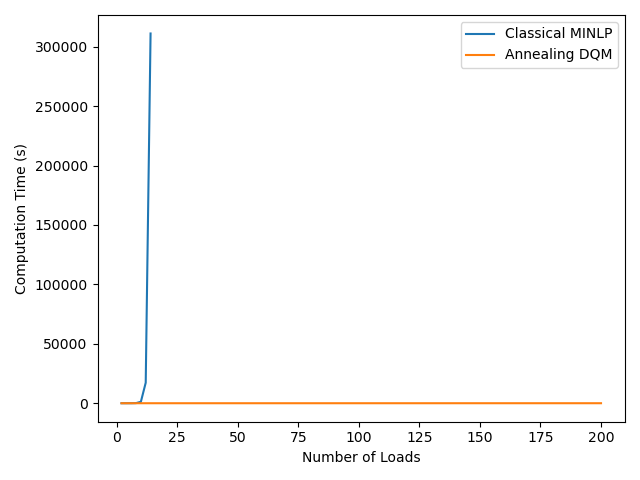
\includegraphics[width=\textwidth]{04_Validation/comparison_performance_c_dqm_p4_extended.png}
    \caption{With up to $200$ Loads}
    \label{figure:validation.comparison.performance.extended}
  \end{subfigure}
  \caption{Performance Comparison of Classical and Hybrid Annealing Algorithms}
\end{figure}


\chapter{Conclusion}

This work proposes an approach to reformulate UCPs with inter-time dependencies as problems that quantum computers can solve.
DQMs and QUBOs are the names of the optimization problems that this approach produces.
Gate-based quantum computers can't optimize the resulting QUBOs because they lack qubits.
Annealing-based quantum computers can't optimize the resulting QUBOs directly on the QPU because they lack connections between their qubits.
But hybrid approaches using both classical computing and quantum computing can optimize the resulting QUBOs and DQMs.

This work compares the performance of hybrid annealing-based optimization of DQMs with the classical optimization of MINLPs for real-world like UCPs.
The hybrid algorithm has a big computational advantage regarding the time it needs to optimize the UCP.
But also, it has a computational disadvantage regarding the quality of the result.
That leads to a trade-off between computation time and optimality of the result.

\section{Future Work}

\subsection{Unit Commitment Problem as Discrete Quadratic Model}

The conversion of the MINLP formulation of the UCP to a DQM formulation is not optimal.
While converting the UCP to a DQM, the proposed approach loses the ability to find the actual optimal solution to the UCP.
This is shown experimentally in section \ref{evaluation:comparison}.

There might be a better way to formulate a DQM for the UCP.
If there is a way that produces DQMs of the same size, it can achieve the same computational advantage as demonstrated in section \ref{evaluation:comparison} while finding the actual optimal solution.
The size of the DQM depends on the number of variables, their possible values, and the number of biases.

\subsection{Using Near-Optimal Result as Input for Classical Optimization}

The classical algorithm for optimizing MINLPs this work considers, ''Couenne'', can have a starting point for the optimization.
The result generated by the hybrid annealing-based DQM sampler could be used as this input.
The idea is to use the hybrid DQM sampler for the global optimization of starting and shutting down power plants and using the classical algorithm for the details of how much energy every plant should generate exactly.

\subsection{Hybrid Mixed-integer Non-linear Problem Solver}

Another promising approach is to find a hybrid algorithm for optimizing MINLP problems directly.
Then the reformulation as a DQM would not be necessary while achieving a computational advantage over purely classical algorithms.
\citeauthor{Ajagekar2020} demonstrated hybrid algorithms for similar mathematical optimization problems like the Mixed-integer Linear Problem (MILP).
\cite{Ajagekar2020}

Such a general-purpose hybrid MINLP solver would help not only the energy industry but also many other industries.
Most real-world industry problems can be formulated as an MINLP.
\cite{Belotti2009}
Thus most real-world industry problems could be solved using such a hybrid MINLP solver.



\printbibliography




\pagestyle{empty}
\renewcommand*{\chapterpagestyle}{empty}
\Versicherung
\end{document}
